\documentclass{bachelor_report}

% Додаткові пакети вносіть у цей файл
% Add your packages here
\usepackage{euscript}  
\usepackage{algorithm}
\usepackage{algorithmic}
\usepackage{hyperref}
\usepackage{amsmath,amsfonts,amssymb,bm}
\usepackage{array}


% Додаткові визначення та перевизначення команд вносіть у цей файл
%%% Ó äàíîìó ôàéë³ âèçíà÷àéòå âñ³ íåîáõ³äí³ âàì íîâ³ êîìàíäè TeX
%%% àáî ðîá³òü ïåðåâèçíà÷åííÿ ³ñíóþ÷èõ, íàïðèêëàä...

% Ïåðåâèçíà÷åííÿ ñèìâîëó ïîðîæíüî¿ ìíîæèíè òà çíàê³â "á³ëüøå-äîð³âíþº", "ìåíøå-äîð³âíþº" íà ïðèéíÿò³ ó íàñ
\let\oldemptyset\emptyset
\let\emptyset\varnothing
\let\geq\geqslant
\let\leq\leqslant

% Âèçíà÷åííÿ íîâèõ ìàòåìàòè÷íèõ êîìàíä
\newcommand*{\binsp}[1]{\ensuremath \left\{0, 1\right\}^{#1}}       % {0, 1}^m
\newcommand*{\xor}{\ensuremath \oplus}                              % \xor = (+)
\newcommand*{\GF}[1]{\ensuremath \mathbb F_{#1}}                    % F_n
\newcommand*{\GFgroup}[1]{\ensuremath \mathbb F^{*}_{#1}}           % F^*_n
\newcommand*{\Zring}[1]{\ensuremath \mathbb Z_{#1}}                 % Z_n
\newcommand*{\Zgroup}[1]{\ensuremath \mathbb Z^{*}_{#1}}            % Z^*_n
\newcommand*{\Jset}[1]{\ensuremath \mathbb J_{#1}}                  % J_n
\newcommand*{\Qset}[1]{\ensuremath \mathbb Q_{#1}}                  % Q_n
\newcommand*{\PQset}[1]{\ensuremath \widetilde{\mathbb Q}_{#1}}     % Q~_n
\newcommand*{\cyclic}[1]{\ensuremath \left\langle {#1} \right\rangle}                  % <g>
\newcommand*{\Legendre}[2]{\ensuremath \left( \frac{#1}{#2} \right)}  % ñèìâîë Ëåæàíäðà/ßêîáè
\newcommand*{\compinv}[1]{\ensuremath {#1}^{\left\langle -1 \right\rangle}}  % îáðàòíûé ïî êîìïîçèöèè

% ²íøèé ñïîñ³á âèçíà÷åííÿ ìàòåìàòè÷íîãî îïåðàòîðó
\DeclareMathOperator{\ord}{ord}
\DeclareMathOperator{\lcm}{lcm}
\DeclareMathOperator{\Li}{Li}
\DeclareMathOperator{\Coef}{Coef}
\DeclareMathOperator{\Log}{Log}
\DeclareMathOperator{\Exp}{Exp}
\DeclareMathOperator{\Res}{Res}
\DeclareMathOperator{\charact}{char}
\DeclareMathOperator{\Sym}{Sym}

%%% ...³ òàêå ³íøå

% Відомості про автора роботи
%%% Основные сведения %%%
\newcommand{\reportAuthor}             % ФИО автора
{Балацька Вікторія Віталіївна}
\newcommand{\reportAuthorGroup}        % группа автора
{ФІ-13}
\newcommand{\reportTitle}              % Название (тема исследования)
{Перевірка IND-CCA та IND-CPA стійкості Baby Kyber}
%% використовуйте символ "\par" або "\\" для розбиття назви на декілька рядків



% Починаємо верстку документа
\begin{document}

\setfontsize{14}

% Створюємо титульну сторінку
% Титульный лист
\thispagestyle{empty}

\begin{center}
НАЦІОНАЛЬНИЙ ТЕХНІЧНИЙ УНІВЕРСИТЕТ УКРАЇНИ \par
<<КИЇВСЬКИЙ ПОЛІТЕХНІЧНИЙ ІНСТИТУТ ім. Ігоря СІКОРСЬКОГО>>\par
НАВЧАЛЬНО-НАУКОВИЙ ФІЗИКО-ТЕХНІЧНИЙ ІНСТИТУТ\par

\vspace{40mm}
{\huge Звіт з переддипломної практики\par}

\huge\MakeUppercase{\textbf{\reportTitle}} \par
\end{center}

\vspace{40mm}
\begin{flushright}
Виконала студентка

групи \reportAuthorGroup

\reportAuthor


\end{flushright}

\vspace{50mm}
\begin{center}
{Київ~--- 2025}
\end{center}

\newpage
\thispagestyle{plain}


%% Створюємо зміст    % -- розкоментуйте, якщо зміст вам потрібен
\pagenumbering{gobble}
\tableofcontents
\cleardoublepage
\pagenumbering{arabic}

\setcounter{page}{3}    %!!! -- продумати, як автоматизувати номер сторінки

%% Якщо ви використовуєте зміст, то прослідкуйте, щоб номер сторінки 
%% співпадав із справжнім!

% Створюємо перелік умовних позначень, скорочень і термінів
% Якщо цей розділ вам не потрібен, просто закоментуйте два наступних рядка
\shortings
%!TEX root = ../thesis.tex
% створюємо перелік умовних позначень, скорочень і термінів
\noindent КЕМ --- механізм інкапсуляції ключів (key encaplusation mechanism)\\
IND-CCA ---  нерозрізнення  за допомогою адаптивно вибраного шифрованого тексту (indistinguishability under adaptive chosen ciphertext attack)\\
CCA --- атака за допомогою вибраного шифротексту (chosen ciphertext cttack)\\
IND-CPA --- нерозрізнення за допомогою вибраного відкритого тексту (indistinguishability under chosen plaintext attack) \\
ML-KEM --- механізм інкапсуляції ключів на основі решітки (module-lattice-based key-encapsulation mechanism)\\
MLWE --- модульне навчання на помилках (module learning with errors)\\
PKE --- схема шифрування з відкритим ключем (public-key encryption)\\
LWE --- задача навчання на помилках (learning with errors)\\
FO --- перетворення Фудзісакі-Окамото (Fujisaki-Okamoto transform) \\

% Створюємо вступ
\intro
%!TEX root = ../thesis.tex
% створюємо вступ
Сучасні криптографічні протоколи встановлення ключів стикаються з викликами, зумовленими розвитком квантових обчислень. Традиційні асиметричні схеми, що забезпечують конфіденційність переданих даних, можуть стати вразливими в умовах появи достатньо потужних квантових комп'ютерів, здатних розв'язувати складні криптографічні задачі. У зв'язку з цим активно розвиваються гібридні схеми і протоколи встановлення ключів, що поєднують класичні та постквантові механізми задля досягнення довготривалої безпеки.

Одна із таких схем представлена у статті Joppe Bos, Leo Ducas та інших <<CRYSTALS – Kyber: a CCA-secure module-lattice-based KEM>> \cite{KyberCCA}. Вона пропонує гібридне поєднання класичних та постквантових компонентів для обміну ключами. Однак для практичного впровадження необхідно оцінити безпеку такої конструкції відносно стандартних моделей стійкості, зокрема IND-CCA та IND-CPA.

\textbf{Метою даної переддипломної практики} є реалізація спрощеної версії даної схеми Kyber та її формальна перевірка на відповідність вимогам IND-CCA та IND-CPA. Дослідження спрямоване на виявлення можливих вразливостей та підтвердження криптографічної стійкості отриманої конструкції.

\textbf{Об’єктом дослідження} є процеси оцінки криптографічної стійкості гібридних схем.

\textbf{Предметом дослідження} є методи аналізу стійкості до IND-CPA та IND-CCA атак.

\textbf{Реалізація алгоритму та експериментальні атаки} доступні у відкритому репозиторії за посиланням: 

\url{https://github.com/tOrryV/Practice_DL.git}.



% Додаємо глави
% Якщо ваша робота містить менше або більше глав - модифікуйте наступні 
% рядки відповідним чином
%!TEX root = ../thesis.tex

\chapter{Реалізація спрощеної версії гібридної криптографічної схеми Kyber}
\label{chap:chapter1}  

У цьому розділі розглянуто реалізацію спрощеної версії гібридної криптографічної схеми Kyber~\cite{KyberWebsite}. Для цього спочатку буде проведено короткий огляд загальної схеми КЕМ Kyber, яка є постквантовою криптосистемою стійкість якої ґрунтується на складності розв’язання задачі навчання на помилках (LWE) над модульними решітками. Далі буде розглянуто Baby Kyber – спрощену версію схеми, яка дозволяє проаналізувати основні принципи роботи Kyber у спрощеному вигляді~\cite{babyKyber}. Теоретичне обґрунтування Baby Kyber допоможе зрозуміти його основні компоненти та алгоритми. Нарешті, буде представлена практична реалізація Baby Kyber, включаючи опис використаних криптографічних примітивів, алгоритми обміну ключами та результати тестування.

%%% --------------------------------------------------------
\section{Огляд криптосистеми Kyber}
%%% -------------------------------------------------------- 

Kyber – це постквантова криптографічна схема для обміну ключами, що ґрунтується на задачах решіткової криптографії. Вона була розроблена для забезпечення стійкості до атак квантових комп’ютерів і стала одним із фіналістів конкурсу NIST з постквантової криптографії.  

У цьому підрозділі буде розглянуто загальну схему роботи Kyber, включаючи основні алгоритми генерації ключів, шифрування та розшифрування. Також буде проаналізовано властивості та рівень безпеки Kyber, зокрема її стійкість до криптографічних атак і ефективність у практичному застосуванні.

\subsection*{Загальна схема роботи Kyber}

Kyber є пост-квантовим КЕМ, що використовує відкритий ключ. Ця схема є першою схемою КЕМ, який стандартизовано.  Механізм інкапсуляції ключів Kyber використовує задачу модульного навчання на помилках (MLWE)~\cite{Langlois2012} та складність її розв'язання. Тобто Kyber - це захищений IND-CCA механізм інкапсуляції ключів (KEM), стійкість якого ґрунтується на складності розв'язання задачі навчання на помилках (LWE) над модульними решітками~\cite{KyberWebsite}.  Звичайно, існують аналогічні схеми, які ґрунтуються на неструктурованому MLWЕ, проте ця конструкція має значно більші переваги в ефективності~\cite{Gonzalez2021}.

Для побудови Kyber спершу вводиться IND-CPA-безпечна схема шифрування з відкритим ключем, яка використовується для шифрування повідомлення фіксованої довжини, після цього, використовуючи FO-перетворення, будується IND-CCA2-безпечний КЕМ~\cite{KyberWebsite}.

Структура Kyber ґрунтується на модульній версії схеми шифрування Ring-LWE LPR~\cite{Lyubashevsky2013, Langlois2012} із відкиданням бітів~\cite{Pessl2017}. Цей КЕМ також посилений багатьма поліпшеними реалізаціями схем шифрування на основі решітки, таких як NewHope~\cite{Alkim2016}. У схемах шифрування, що використовуються (NewHope та схемах Ring-LWE) операції мали вигляд $As+e$, де всі ці змінні є поліномами у кільці~\cite{Avanzi2021}. Проте, на відміну від них, Kyber використовує матрицю $A$ над кільцем поліномів, а $s, e$ - це вектори над тим самим кільцем, що і матриця~\cite{Avanzi2021}. Для Kyber $A$ є квадратною матрицею розміру $k\times k$, а вектори $s, e$ є k-вимірними векторами.  

Особливістю Kyber є використання так званого теоретико-числового перетворення (NTT)~\cite{Botros2019}. NTT перетворює поліном $f \in R_q$ в представлення у вигляді вектора $f$ лінійних поліномів~\cite{Botros2019}. Саме це перетворення дозволяє пришвидшити операцію множення поліномів. 


Опис роботи КЕМ та алгоритм поданий нижче, ґрунтується на роботі~\cite{Lyubashevsky2024}.
За допомогою алгоритму KeyGen створюються відкритий та особистий ключі. Спочатку, випадково створюється матриця $A$ із кільця поліномів ${R}_{3329}^{k \times k, X^{256}+1}$ та вектори $s, e$, що використовуються для додавання шуму. У результаті обчислюється значення t, та повертаються необхідні ключі: $pk = (\mathbf{A}, t)$ - відкритий ключ,  $sk = s$ - особистий ключ. За допомогою алгоритму Encrypt, шифрується повідомлення m, використовуючи відкритий ключ pk. Спочатку створюються вектори $r, e_1, e_2$, далі обчислюються значення $u^T$ та $v$. Після виконання алгоритму отримується шифротекст $(u, v)$. За допомогою алгоритму розшифрування відновлюється  повідомлення m використовуючи отриманий шифротекст та особистий ключ sk. Спершу обчислюється значення $u\textquotesingle$ де шифротекст переводиться назад у простір за модулем q та обчислюється значення $v\textquotesingle$ де аналогічно обробляється друга частина шифротексту $v$. У результаті обчислення $m\textquotesingle$ отримується повідомлення $m$. 

\begin{algorithm}[H]
	\caption{Kyber Encryption Scheme}
	
	\textbf{KeyGen:}\\
		 Generate $\mathbf{A} \leftarrow \mathcal{R}_{3329}^{k \times k, X^{256}+1}$\\
		 Sample $(s, e) \leftarrow \psi_{\eta_1}^k \times \psi_{\eta_1}^k$\\
		Compute $t := \mathbf{A}s + e$\\
		Output $pk = (\mathbf{A}, t)$ and $sk = s$\\
	
	\textbf{Encrypt ($pk = (\mathbf{A}, t), m$):}\\
		Sample $(r, e_1, e_2) \leftarrow \psi_{\eta_1}^k \times \psi_{\eta_1}^k \times \psi_{\eta_2}$\\
		 Compute $\mathbf{u}^T := \big[\mathbf{r}^T \mathbf{A} + e_1^T \big]_{q \to 2^{d_u}}$\\
		Compute $v := \big[\mathbf{r}^T t + e_2 + \frac{q-1}{2} m \big]_{q \to 2^{d_v}}$\\
		Output $\text{ciphertext} = (\mathbf{u}, v)$\\
	
	\textbf{Decrypt ($sk = s, \text{ciphertext} = (\mathbf{u}, v)$):}\\
		Recover $\mathbf{u}' := [\mathbf{u}]_{2^{d_u} \to q}$\\
		 Recover $v' := [v]_{2^{d_v} \to q}$\\
		 Compute $m' := \big[v' - \mathbf{u}'^T s \big]_{q \to 2}$\\
		Output $m'$\\
	
\end{algorithm}



\subsection*{Властивості Kyber}

1. Параметри та рівні безпеки Kyber:

Kyber має три основні варіанти параметрів, кожен з яких відповідає певному рівню криптографічної стійкості~\cite{babyKyber}. Рівень безпеки визначається відповідно до стійкості класичних криптографічних алгоритмів, таких як AES та RSA, до атак квантових комп'ютерів.
\begin{enumerate}
    \item Kyber512: орієнтований на рівень безпеки, еквівалентний AES-128.
    \item Kyber768: відповідає рівню безпеки AES-192.
    \item Kyber1024: забезпечує рівень безпеки, подібний до AES-256.
\end{enumerate}

\textbf{Kyber512}

Kyber512 є найменшою конфігурацією у сімействі Kyber і забезпечує рівень безпеки, еквівалентний AES-128. Він був розроблений для ефективного постквантового обміну ключами з використанням решіткової криптографії~\cite{KyberWebsite}.

Основні параметри~\cite{KyberWebsite}:
\begin{itemize}
    \item Рівень безпеки: аналог AES-128
    \item Розмір відкритого ключа: 800 байтів
    \item Розмір особистого ключа: 1632 байти
    \item Розмір шифротексту: 768 байтів
\end{itemize}

\textbf{Kyber768}

Kyber768 – це середній рівень безпеки в сімействі CRYSTALS-Kyber, призначений для відповідності AES-192 у класичній криптографії. Він має покращені параметри порівняно з Kyber512, що підвищує його стійкість, але водночас збільшує розмір ключів і шифротекстів~\cite{KyberWebsite}.

Основні параметри~\cite{KyberWebsite}:
\begin{itemize}
    \item Рівень безпеки: аналог AES-192
    \item Розмір відкритого ключа: 1184 байтів
    \item Розмір особистого ключа: 2400 байти
    \item Розмір шифротексту: 1088 байтів
\end{itemize}

\textbf{Kyber1024}

Kyber1024 – це найвищий рівень безпеки в сімействі CRYSTALS-Kyber, розроблений для відповідності AES-256 у класичній криптографії. Він має ще більші параметри, що забезпечує максимальну стійкість серед усіх варіантів Kyber, але водночас збільшує розмір ключів та шифротекстів.~\cite{KyberWebsite}.

Основні параметри~\cite{KyberWebsite}:
\begin{itemize}
    \item Рівень безпеки: аналог AES-256
    \item Розмір відкритого ключа: 1568 байтів
    \item Розмір особистого ключа: 3168 байти
    \item Розмір шифротексту: 1568 байтів
\end{itemize}

\subsection*{Безпека Kyber}

Алгоритми сімейства Kyber (512, 768, 1024) використовують схему гібридного шифрування на основі Module-LWE (MLWE). Всі три варіанти забезпечують IND-CPA стійкість на базовому рівні, а IND-CCA стійкість завдяки трансформації Fujisaki-Okamoto (FO)~\cite{KyberNISTRound3}.

1. IND-CPA стійкість~\cite{ScienceDirect2023}
\begin{enumerate}[label=\alph*)]
    \item IND-CPA гарантується випадковими шумовими компонентами в обчисленнях.
    \item Використання MLWE-складності унеможливлює ефективний аналіз шифротекстів навіть для квантових алгоритмів.
    \item Всі варіанти Kyber забезпечують IND-CPA стійкість без додаткових трансформацій.
\end{enumerate}

2. IND-CCA стійкість~\cite{KyberCCA}
\begin{enumerate}[label=\alph*)]
    \item IND-CCA досягається за допомогою перетворення Фудзісакі Окамотто.
    \item Це перетворення включає повторну інкапсуляцію та перевірку правильності шифротексту, що запобігає обманним запитам на дешифрування.
    \item Усі три версії Kyber використовують FO-перетворення для забезпечення IND-CCA стійкості.
\end{enumerate}

%%% --------------------------------------------------------
\section{Теоретична реалізація Baby Kyber}
%%% --------------------------------------------------------

У цьому підрозділі буде розглянуто спрощену версію криптосистеми Kyber, відому як Baby Kyber. Ця модель зберігає основні ідеї оригінальної схеми, але використовує зменшені параметри, що робить її зручнішою для аналізу та розуміння.  

Спочатку буде описано принципи спрощення схеми Kyber, які дозволяють отримати Baby Kyber. Далі розглянемо основні математичні операції, що використовуються у цій криптосистемі, зокрема операції в кільцях та роботу з многочленами. Потім буде детально описано алгоритми генерації ключів, шифрування та розшифрування, які є основою роботи Baby Kyber.  

\subsection*{Спрощення схеми Kyber}

Для полегшення аналізу криптосистеми Kyber створюється її спрощена версія — Baby Kyber. Вона зберігає основні криптографічні принципи Kyber, але використовує зменшені параметри та спрощені математичні операції~\cite{babyKyber}. Спрощення полягає у: 

1) Зменшення розміру параметрів: у стандартній версії Kyber використовується кільце поліномів ${R}_{n}^{k \times k, X^{n}+1}$, де $n = 512/768/1024$, $q$~-~велике просте число. У версії Baby Kyber використовують зменшені значення параметрів (наприклад $n$ до 4 чи 8) та використовують менші значення модуля $q$ (наприклад 97, замість 3329).

2) Використання малих поліномів в особистому ключі: секретний ключ складається з поліномів із малими коефіцієнтами, що полегшує їх генерацію та обробку.

3) Спрощена матриця $A$: у стандартному Kyber використовується випадкова матриця А розміру $k\times k$. У Baby Kyber використовується фіксована одномірна матриця $A$, що значно спрощує генерацію публічного ключа.

4) Відсутність перетворення Фудзісакі Окамотто: У стандартному Kyber використовується FO-перетворення, яке підсилює схему, роблячи її стійкою до атаки з вибором шифротексту. У Baby Kyber відсутнє FO-перетворення, тому ця схема не має IND-CCA стійкості та ближча до базової форми шифрування на решітках.

5) Відсутність NTT перетворення (Number Theoretic Transform): У стандартному Kyber для ефективного множення поліномів використовується NTT-перетворення, яке суттєво прискорює обчислення у великому полі. У Baby Kyber NTT не використовується, а всі обчислення виконуються напряму в кільці, що робить реалізацію простішою, але менш ефективною.

\subsection*{Основні математичні операції у Baby Kyber}
У Baby Kyber використовуються основні математичні операції, які є спрощеною версією тих, що застосовуються у повноцінному Kyber. Основні операції включають:

1) Додавання поліномів: операція додавання в Baby Kyber здійснюється через покомпонентне додавання коефіцієнтів двох поліномів за модулем $q$, де $q$ є малим простим числом. Після цього результат доцільно взяти за модулем $x_n + 1$, щоб зменшити результати на рівні поліномів.
$$p_1(x)+p_2(x) = \big(\sum^{n-1}_{i=0}(p_{1,i}+p_{2,i}) \mod q\big) \mod (x^n+1)$$

2) Множення поліномів: множення поліномів також виконується за допомогою покомпонентного множення коефіцієнтів двох поліномів, з наступним зведенням результату за модулем $q$. Після цього результат беремо за модулем $x_n + 1$, щоб зменшити степінь полінома. 
$$p_1(x)\cdot  p_2(x) = \sum^{n-1}_{i=0}\big(\sum^{n-1}_{j=0}(p_{1,i} \cdot p_{2,j}) \mod q\big) \mod (x^n+1)$$

3) Редукція полінома за модулем $x_n + 1$: редукція поліномів виконується за допомогою операції зменшення степеня полінома в кільці.  Це означає, що при наявності степеня полінома, який перевищує $n - 1$, відбувається заміна вищих степенів 
$x^n, x^{n+1}, ...$ на відповідні вирази, які зберігають коректність у межах кільця. 
$$p(x) \mod (x^n+1)= \sum^{n-1}_{i=0}(p_i \mod q)  $$

4) Генерація випадкових поліномів: У Baby Kyber випадкові поліноми генеруються з коефіцієнтами, які мають певний набір значень. Ці поліноми використовуються для генерації секретних і публічних ключів.

\subsection*{Алгоритми генерування ключів, шифрування та розшифрування}

1) Генерування ключів

\textit{Відкритий ключ}: відкритий ключ складається із двох компонентів: випадкова матриця $A$ та випадковий вектор $t$.
\begin{enumerate}[label=\alph*)]
    \item Матриця $A$: це матриця розміру $k\times k$,  де кожен елемент є випадковим поліномом з кільця $\mathbb{Z}_q[X]/(X^n+1)$. Кожен коефіцієнт полінома вибирається випадково з проміжку $[0, q - 1]$

    \item Вектор $t$: це вектор розміру $k$, де кожен компонент обчислюється як $A\cdot s + e$, де $s$ - особистий ключ, $e$ - вектор шуму. Вектори $s$ та $e$ також складаються з поліномів, згенерованих через центральний біноміальний розподіл (CBD).
\end{enumerate}

\textit{Особистий ключ}: особистий ключ складається з випадкового вектора поліномів $s$, що з генерується малими значеннями та шуму $e$, що додається для забезпечення стійкості до атак.

2) Шифрування

Шифрування виконується за алгоритмом з використанням відкритого ключа $(A, t)$:
\begin{enumerate}[label=\alph*)]
    \item Вибір випадковий поліномів: генеруються два набори випадкових поліномів $r$ та $e_1$ для шуму, вибраних за допомогою центрального біноміального розподілу (CBD).Також генерується випадковий поліно $e_2$ для додаткового шуму в шифротексті. 

    \item Компонентами шифротексту є вектори $u$ та $v$. Для створення кожного елемента вектора $u$, проводиться множення кожного стовпця транспонованої матриці $A^T$ на відповідний поліном вектора $r$,  після чого додається шум $e_1$
    Компоненту $v$ обчислюють за допомогою додавання поліномів $e_2$ та результату множення кожного елемента вектора $t$ на відповідний елемент вектора $r$. Після цього додається масштабоване повідомлення $m$, яке є поліномом, що представляє бітове повідомлення. Кожен біт повідомлення множиться на $\lceil q/2 \rceil$.

    \item В результаті шифротекст складається із двох компонент $(u, v)$, які разом містять зашифроване повідомлення. 
\end{enumerate}

2) Розшифрування

Розшифрування за допомогою секретного ключа $s$ відбувається наступним чином:
\begin{enumerate}[label=\alph*)]
    \item Обчислення скалярного добутку $s^Tu$. Тут кожен елемент вектора $s$ множиться на відповідний елемент вектора $u$, а потім ці добутки додаються.

    \item Для отримання розшифрованого результату спочатку розшифроване значення $v$ зменшується на $s^Tu$. Для отримання бітів повідомлення, кожен коефіцієнт результату розшифровки зменшується за модулем $q$, а потім порівнюється з межами для визначення, чи є це 1 або 0 в оригінальному повідомленні. 

    \item Після перевірки кожного коефіцієнта результату розшифрування формується вектор бітів m, який представляє оригінальне повідомлення.
\end{enumerate}



%%% --------------------------------------------------------
\section{Практична реалізація Baby Kyber}
%%% --------------------------------------------------------
У цьому розділі буде розглянуто практичну реалізацію Baby Kyber. Спочатку буде обґрунтовано вибір середовища розробки та необхідних інструментів, які забезпечують зручність роботи з многочленами та криптографічними операціями. Далі буде подано опис основних функцій реалізації, включаючи операції над поліномами, генерацію ключів, шифрування та розшифрування. На завершальному етапі буде проведено перевірку коректності реалізованих алгоритмів та тестування для оцінки їхньої відповідності теоретичним очікуванням.

\subsection*{Вибір середовища розробки та інструментів} 

Для реалізації алгоритму Baby Kyber було обрано мову програмування Python. Основними причинами такого вибору є:

1. Зручність написання та читабельність коду: Python має лаконічний синтаксис, який полегшує розуміння та підтримку коду. Це особливо важливо в криптографії, де складність алгоритмів висока, і зрозумілий код спрощує налагодження та аналіз безпеки.  

2. Вбудовані бібліотеки та підтримка великих чисел:  Python підтримує довільну точність цілих чисел, що є критично важливим для криптографічних алгоритмів, які працюють з великими просторами модулів. Також стандартна бібліотека **math** забезпечує всі необхідні операції для роботи з модулярною арифметикою.  

3. Можливість швидкої розробки та прототипування:  у криптографії часто необхідно тестувати різні підходи та параметри. Python дозволяє швидко реалізовувати нові ідеї та перевіряти їхню ефективність без необхідності компіляції та складного керування пам’яттю.  

4. Наявність криптографічних бібліотек:  хоча Baby Kyber реалізується вручну, Python має низку бібліотек для криптографії (PyCryptodome, cryptography, hashlib), які можуть допомогти у створенні допоміжних інструментів, тестуванні та порівнянні з іншими алгоритмами.  

5. Гнучкість та переносність: код на Python можна запускати на різних операційних системах без значних змін, що спрощує тестування та використання алгоритму в різних середовищах.  

Для реалізації обрано середовище розробки PyCharm, оскільки воно надає низку переваг, які спрощують процес розробки, тестування та налагодження коду. Воно пропонує:

1. Інтелектуальне автодоповнення коду: PyCharm має потужний механізм автодоповнення коду, який допомагає швидше писати та редагувати код, зменшуючи кількість помилок і підвищуючи продуктивність.  

2. Інтегрований налагоджувач (debugger): криптографічні алгоритми можуть бути складними у відлагодженні через багатоетапні обчислення. Вбудований debugger дозволяє покроково аналізувати виконання коду, перевіряти значення змінних та знаходити помилки без потреби у вставленні додаткових `print()`.   

3. Зручна інтеграція з Git: у процесі розробки важливо використовувати систему контролю версій Git. PyCharm надає графічний інтерфейс для роботи з Git, що спрощує управління комітами, створення гілок та аналіз історії змін.  

4. Інтегрована консоль та термінал: PyCharm містить вбудований термінал, що дозволяє запускати скрипти, тестувати код і виконувати команди без потреби перемикатися між вікнами.  
 
5. Кросплатформеність: PyCharm доступний для Windows, macOS і Linux, що робить його зручним для роботи на будь-якій операційній системі.  

Для реалізації алгоритму використовуються наступні бібліотеки Python:

1. math: ця стандартна бібліотека Python надає математичні функції, які використовуються для операцій над числами, округлення, піднесення до степеня та обчислення модулів. У криптографічних алгоритмах часто потрібні обчислення залишків, роботи з великими числами та логарифми.

2. secrets: бібліотека secrets використовується для генерації криптографічно стійких випадкових чисел. Це критично важливо для криптографічних алгоритмів, оскільки використання звичайної random може зробити систему вразливою для атак.

\subsection*{Опис основних функцій реалізації}

\textbf{Клас $RingPolynomOperations$}

Цей клас $RingPolynomOperations$ реалізує операції з поліномами в кільці $\mathbb{Z}_q[X] / (X^n + 1)$, що є важливим для криптосистеми Baby Kyber. Він включає методи для додавання та множення поліномів, а також для їх редукції.

\begin{enumerate}
    \item Метод $init$ ініціалізує об'єкт класу з параметрами:
    \begin{enumerate}
        \item $mod$: модуль для виконання операцій.
        \item $n$: ступінь полінома.
    \end{enumerate}

    \item Метод $add$ додає два поліноми покомпонентно за модулем $mod$, після чого виконує редукцію за $X^n + 1$.

    \item Метод $multiply$ обчислює добуток двох поліномів з подальшою редукцією за $X^n + 1$ та модулем $mod$.

    \item Метод $module$ виконує редукцію полінома за $X^n + 1$, коригуючи коефіцієнти та приводячи їх до значень за модулем $mod$.
\end{enumerate}


Цей клас забезпечує базові операції для маніпулювання поліномами у криптосистемах, де поліноми мають бути оброблені за модулем конкретного числа, а також з обмеженням на їх ступінь.


\textbf{Клас $BabyKyber$}

Клас $BabyKyber$ реалізує криптосистему Baby Kyber, що є спрощеною версією алгоритму Kyber. Цей клас включає методи для генерації ключів, шифрування та дешифрування повідомлень. Основною особливістю є використання поліномів і центрованого біноміального розподілу (CBD) для генерації шуму.
\begin{enumerate}
    \item Метод $init$ ініціалізує об'єкт класу з параметрами:
    \begin{enumerate}
        \item $n$: ступінь полінома.
        \item $eta$: параметр для контролю рівня шуму, що генерується.
        \item $k$: розмірність матриці.
        \item $q$: модуль для виконання операцій.
        \item $ring$: об'єкт класу $RingPolynomOperations$, який надає функції для операцій над поліномами.
    \end{enumerate}

    \item Метод $sample\_uniform\_polynomial$ генерує випадковий поліном з коефіцієнтами, вибраними рівномірно з діапазону $[0, q-1]$. Ступінь полінома не перевищує значення $degree$.

    \item Метод $sample\_cbd\_polynomial$ генерує поліном, коефіцієнти якого вибрані за допомогою центрованого біноміального розподілу (CBD). Кожен коефіцієнт обчислюється як різниця двох випадкових значень з рівномірного розподілу на $[0, eta]$. Поліном редукується за модулем $X^n + 1$.
    
    \item Метод $key\_gen$ генерує відкритий і особистий ключі для криптосистеми Baby Kyber.

    \item Метод $encrypt$ шифрує повідомлення, використовуючи відкритий ключ $(A,t)$.
    
     \item Метод $decrypt$ дешифрує шифротекст $(u,v)$ за допомогою особистого ключа $s$.

\end{enumerate}

\textbf{Main файл}

Main файл є основним компонентом для реалізації криптосистеми Baby Kyber.
\begin{enumerate}
    \item Функція $text\_to\_bits$ перетворює текст у список бітів.

    \item Функція $bits\_to\_text$ відновлює текст із списку бітів.

    \item Функція $encrypt\_text$ виконує шифрування. Вона ділить вхідні біти на блоки довжини $n$. Далі додає нулі до блоку, якщо його довжина менша за $n$ і використовує алгоритм BabyKyber для шифрування кожного блоку.

    \item Функція $decrypt\_text$ виконує розшифрування. Вона використовує алгоритм BabyKyber для розшифрування кожного блоку. Після чого об'єднує всі розшифровані біти у список та перетворює його у текст.

    \item Функція $main$ організовує виконання програми:
    \begin{itemize}
        \item Визначає параметри криптосистеми ($q$, $n$, $k$, $\eta$).
        \item Ініціалізує кільцеві операції та алгоритм BabyKyber.
        \item Генерує ключі: відкриту матрицю $A$, відкритий вектор $t$ та секретний вектор $s$.
        \item Перетворює повідомлення у біти.
        \item Виконує шифрування та виводить шифротекст.
        \item Виконує розшифрування та виводить отримане повідомлення.
        \item Перевіряє правильність розшифрування.
    \end{itemize}
\end{enumerate}

\subsection*{Перевірка коректності та тестування}

\textbf{Результати виконання}
\begin{figure}[h]
    \centering
    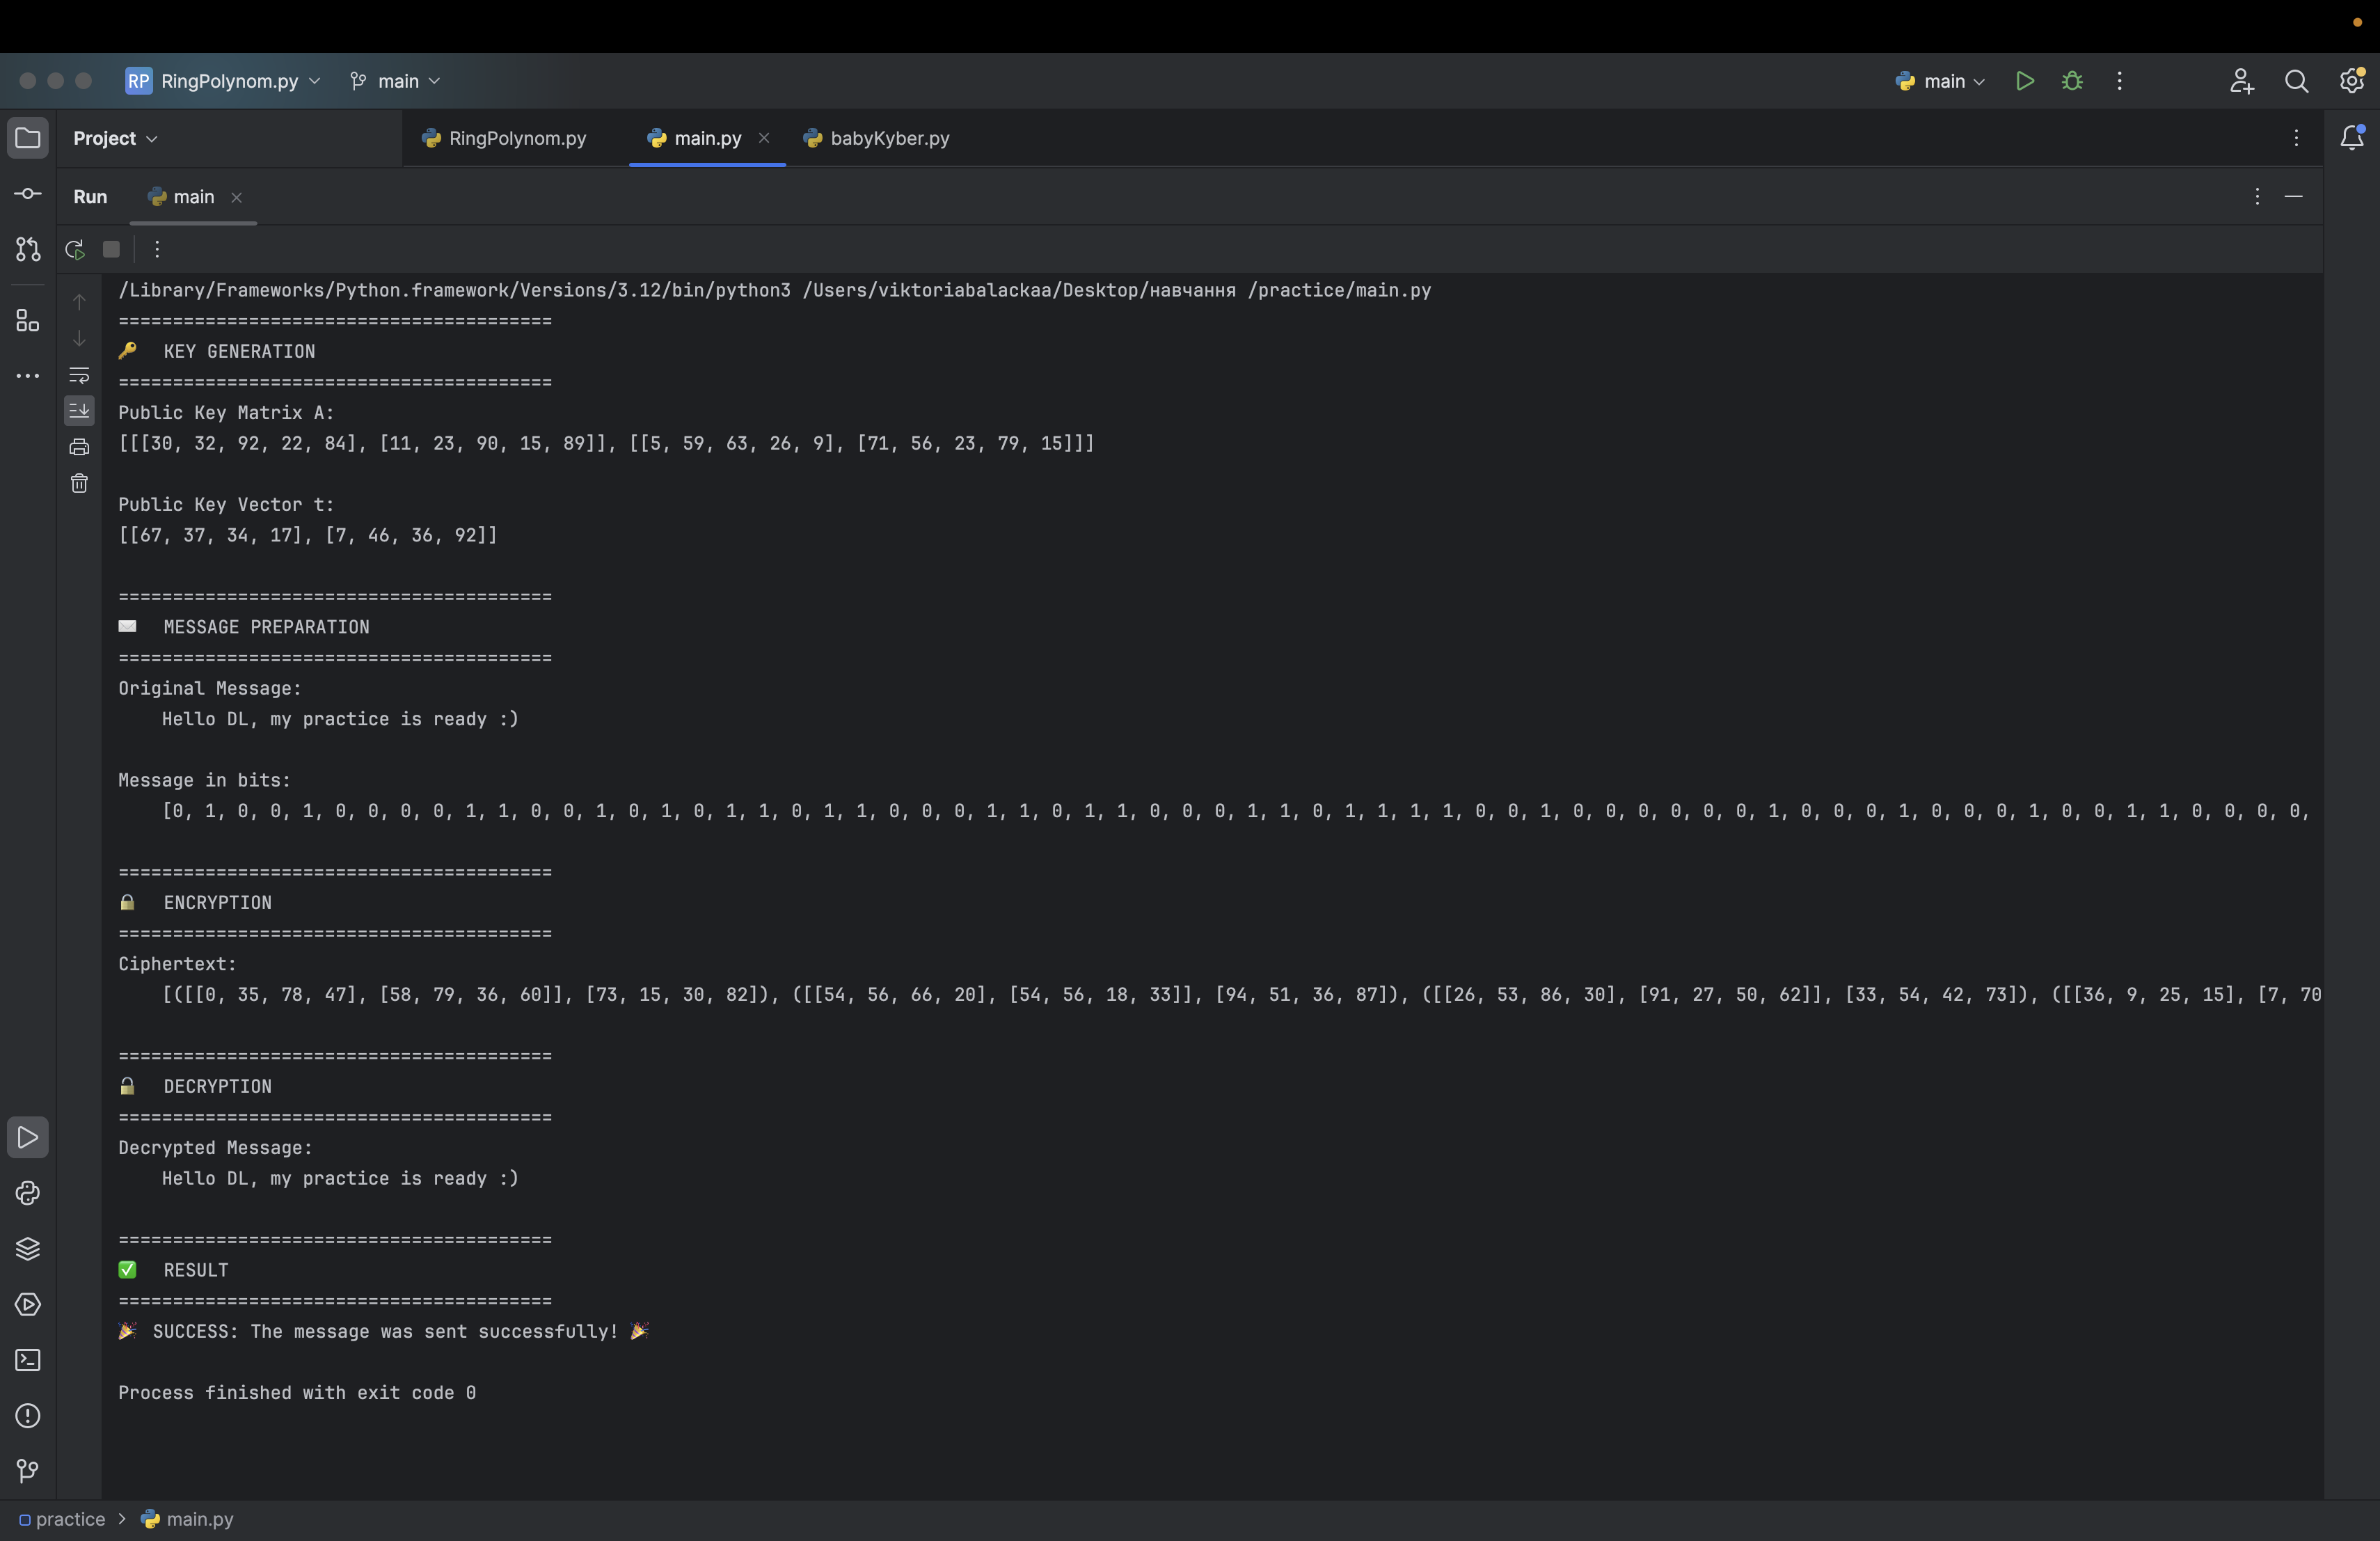
\includegraphics[width=\textwidth]{ПРАКТИКА/Images/test_1.png}
    \caption{Результат 1}
\end{figure}

\begin{figure}[h]
    \centering
    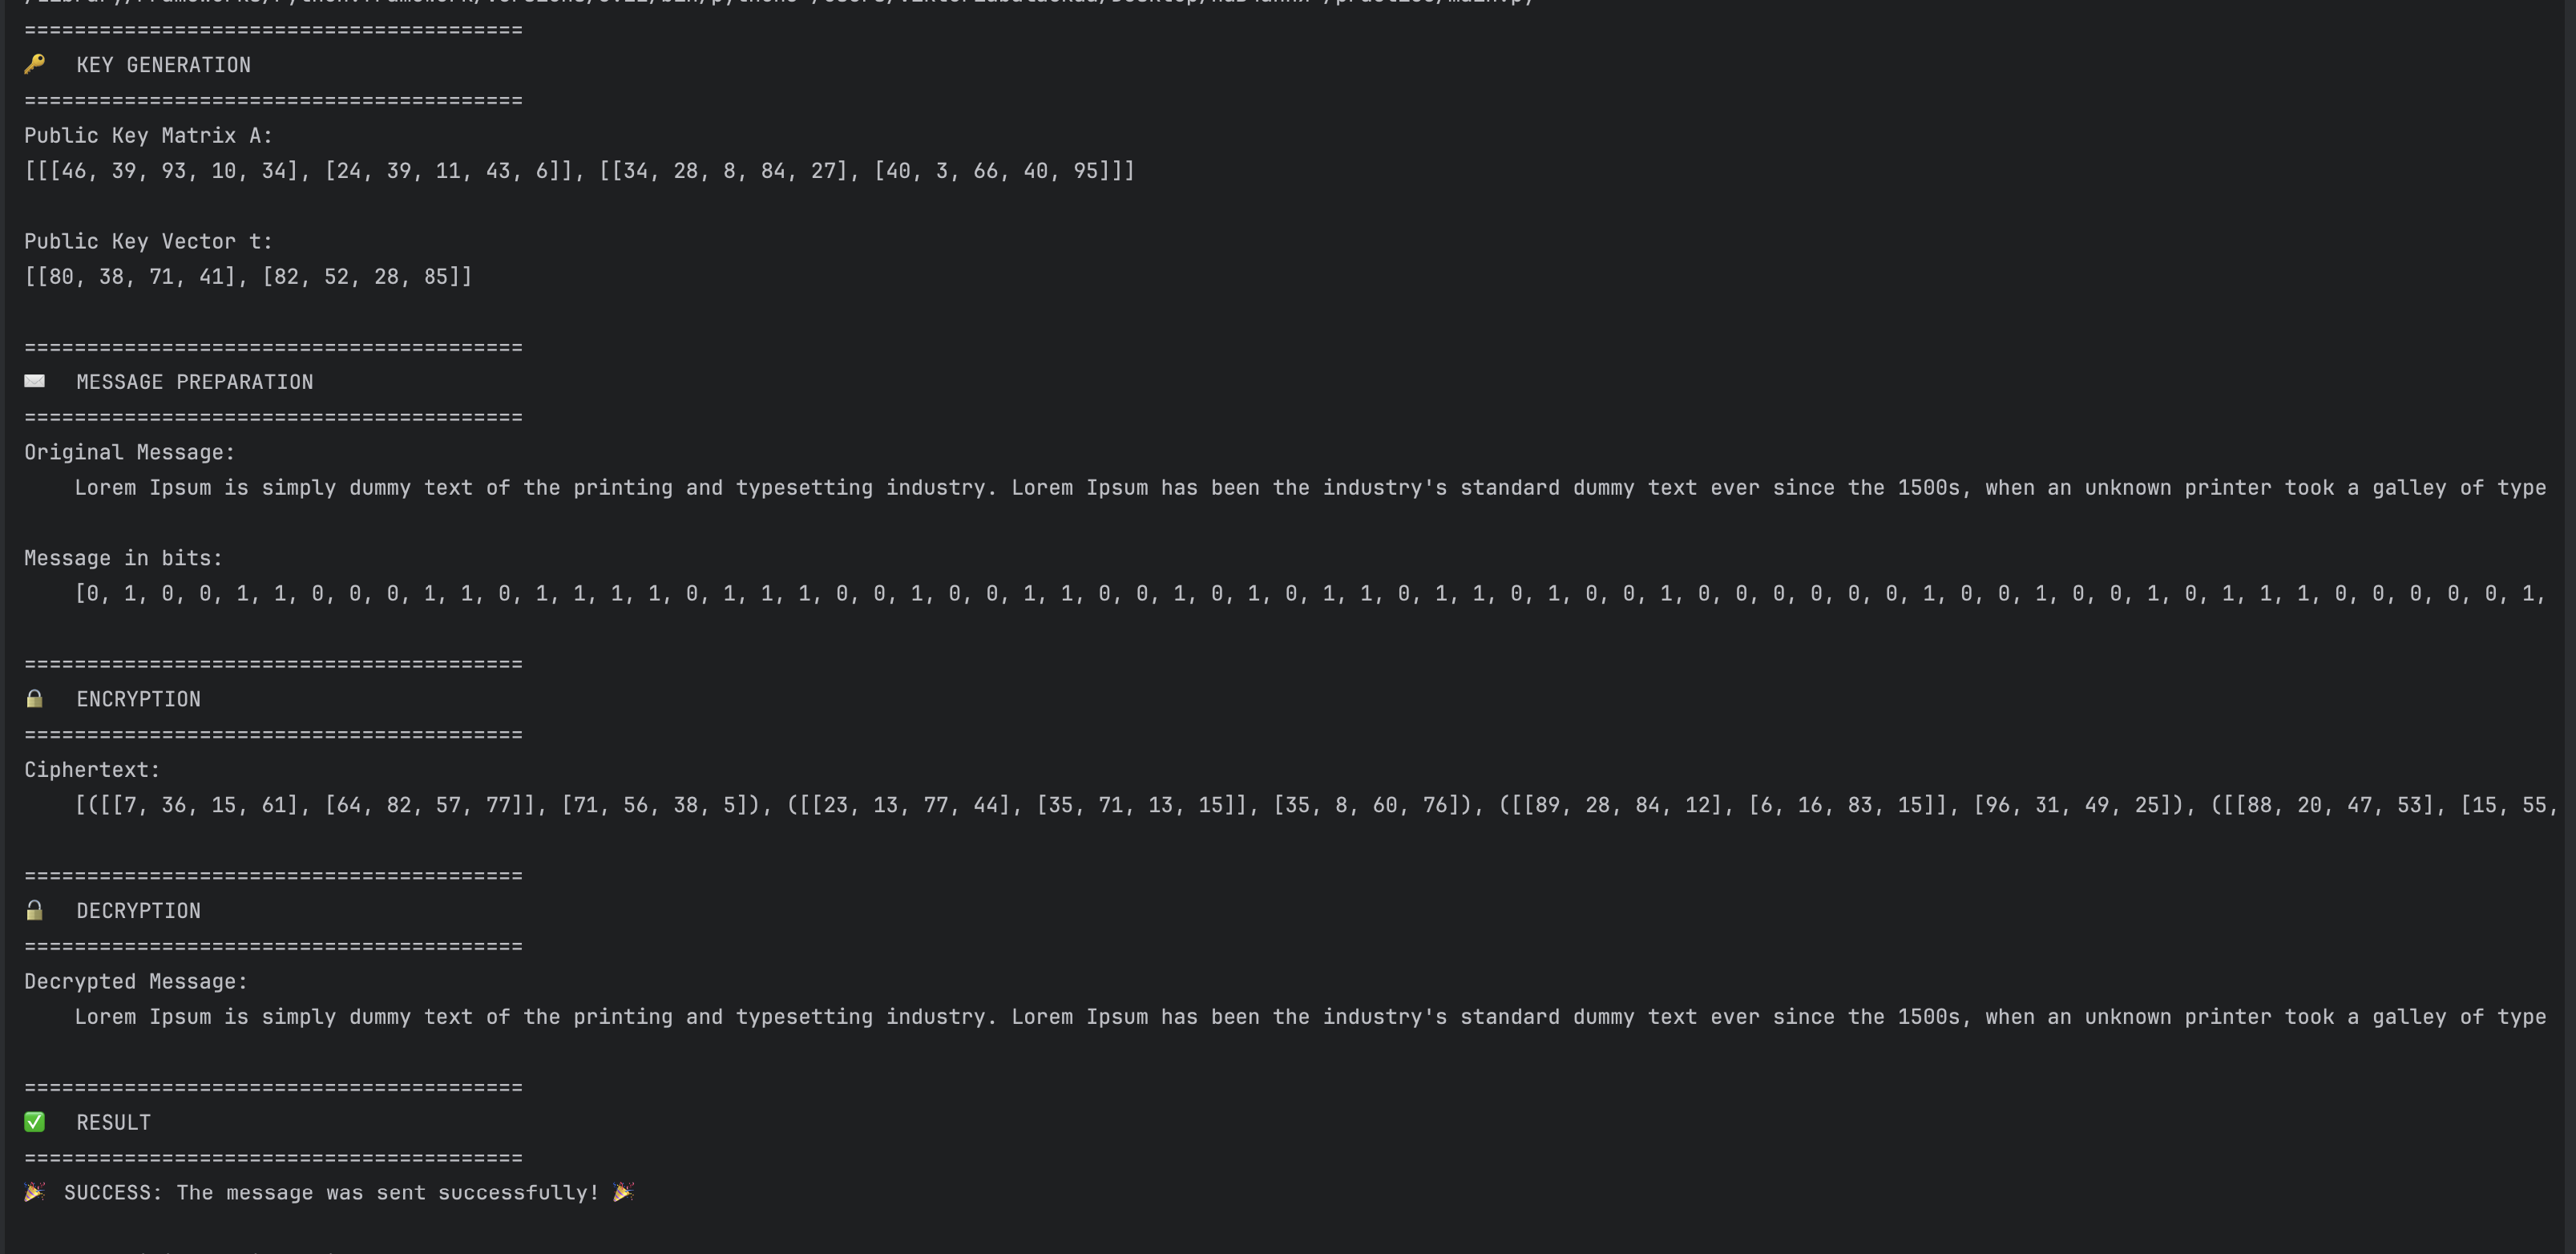
\includegraphics[width=\textwidth]{ПРАКТИКА/Images/test_2.png}
    \caption{Результат 2}
\end{figure}

\begin{figure}[h]
    \centering
    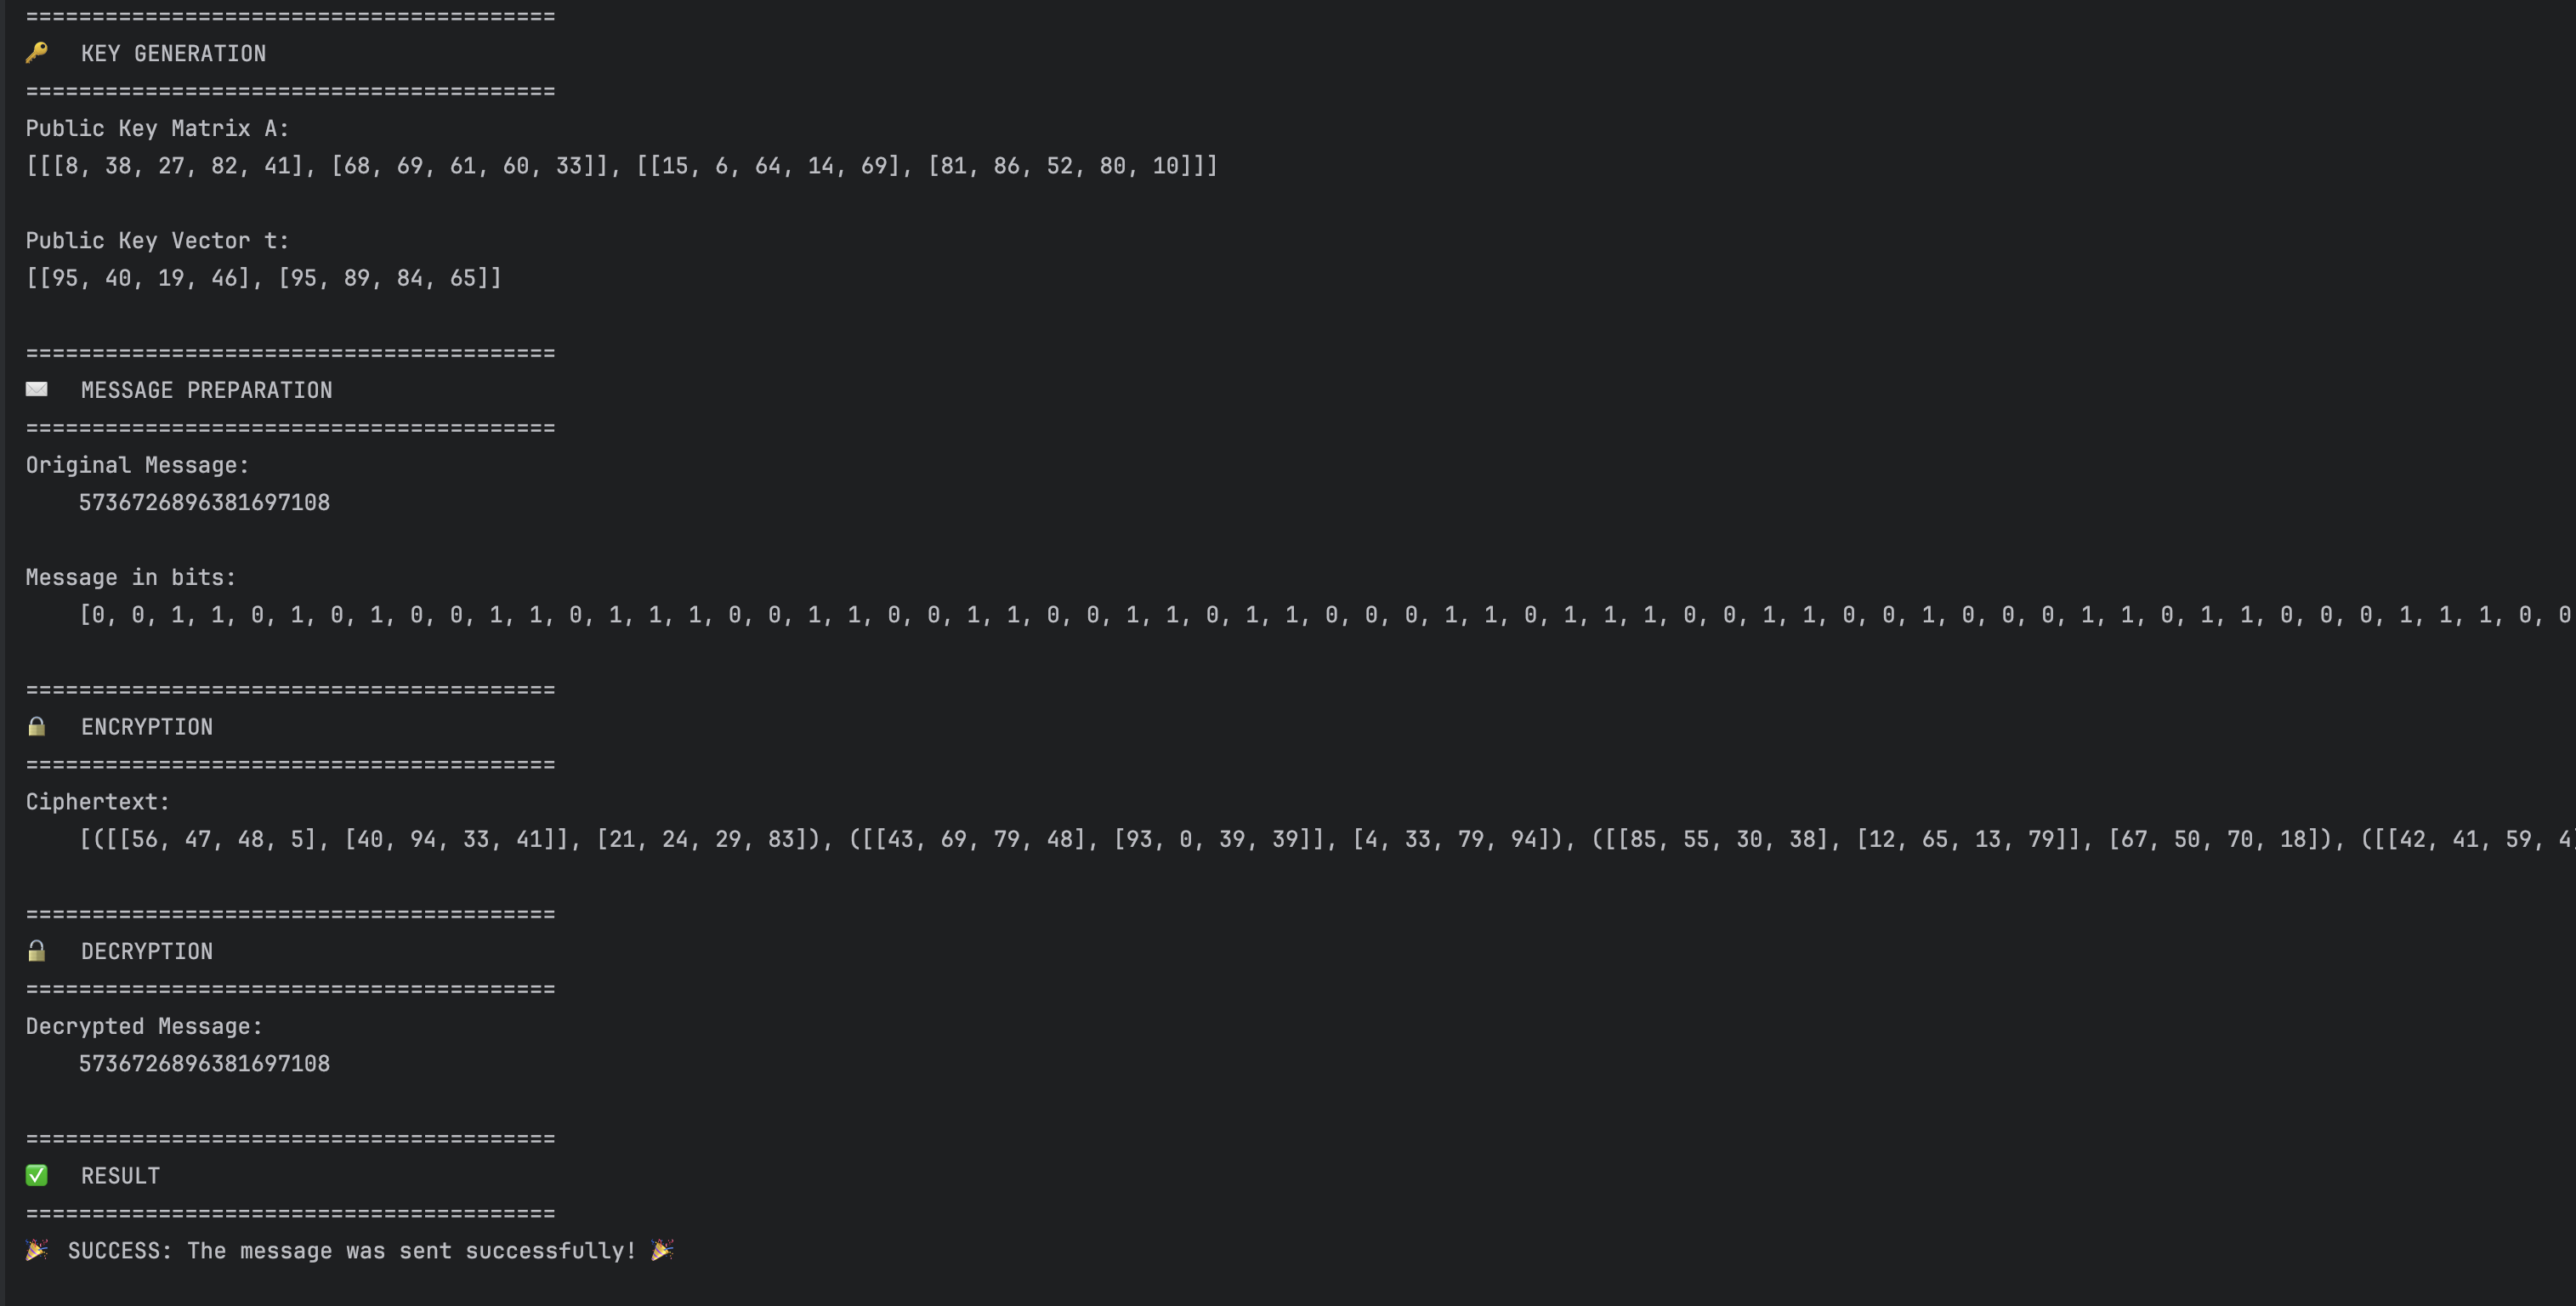
\includegraphics[width=\textwidth]{ПРАКТИКА/Images/test_3.png}
    \caption{Результат 3}
\end{figure}

\begin{figure}[h]
    \centering
    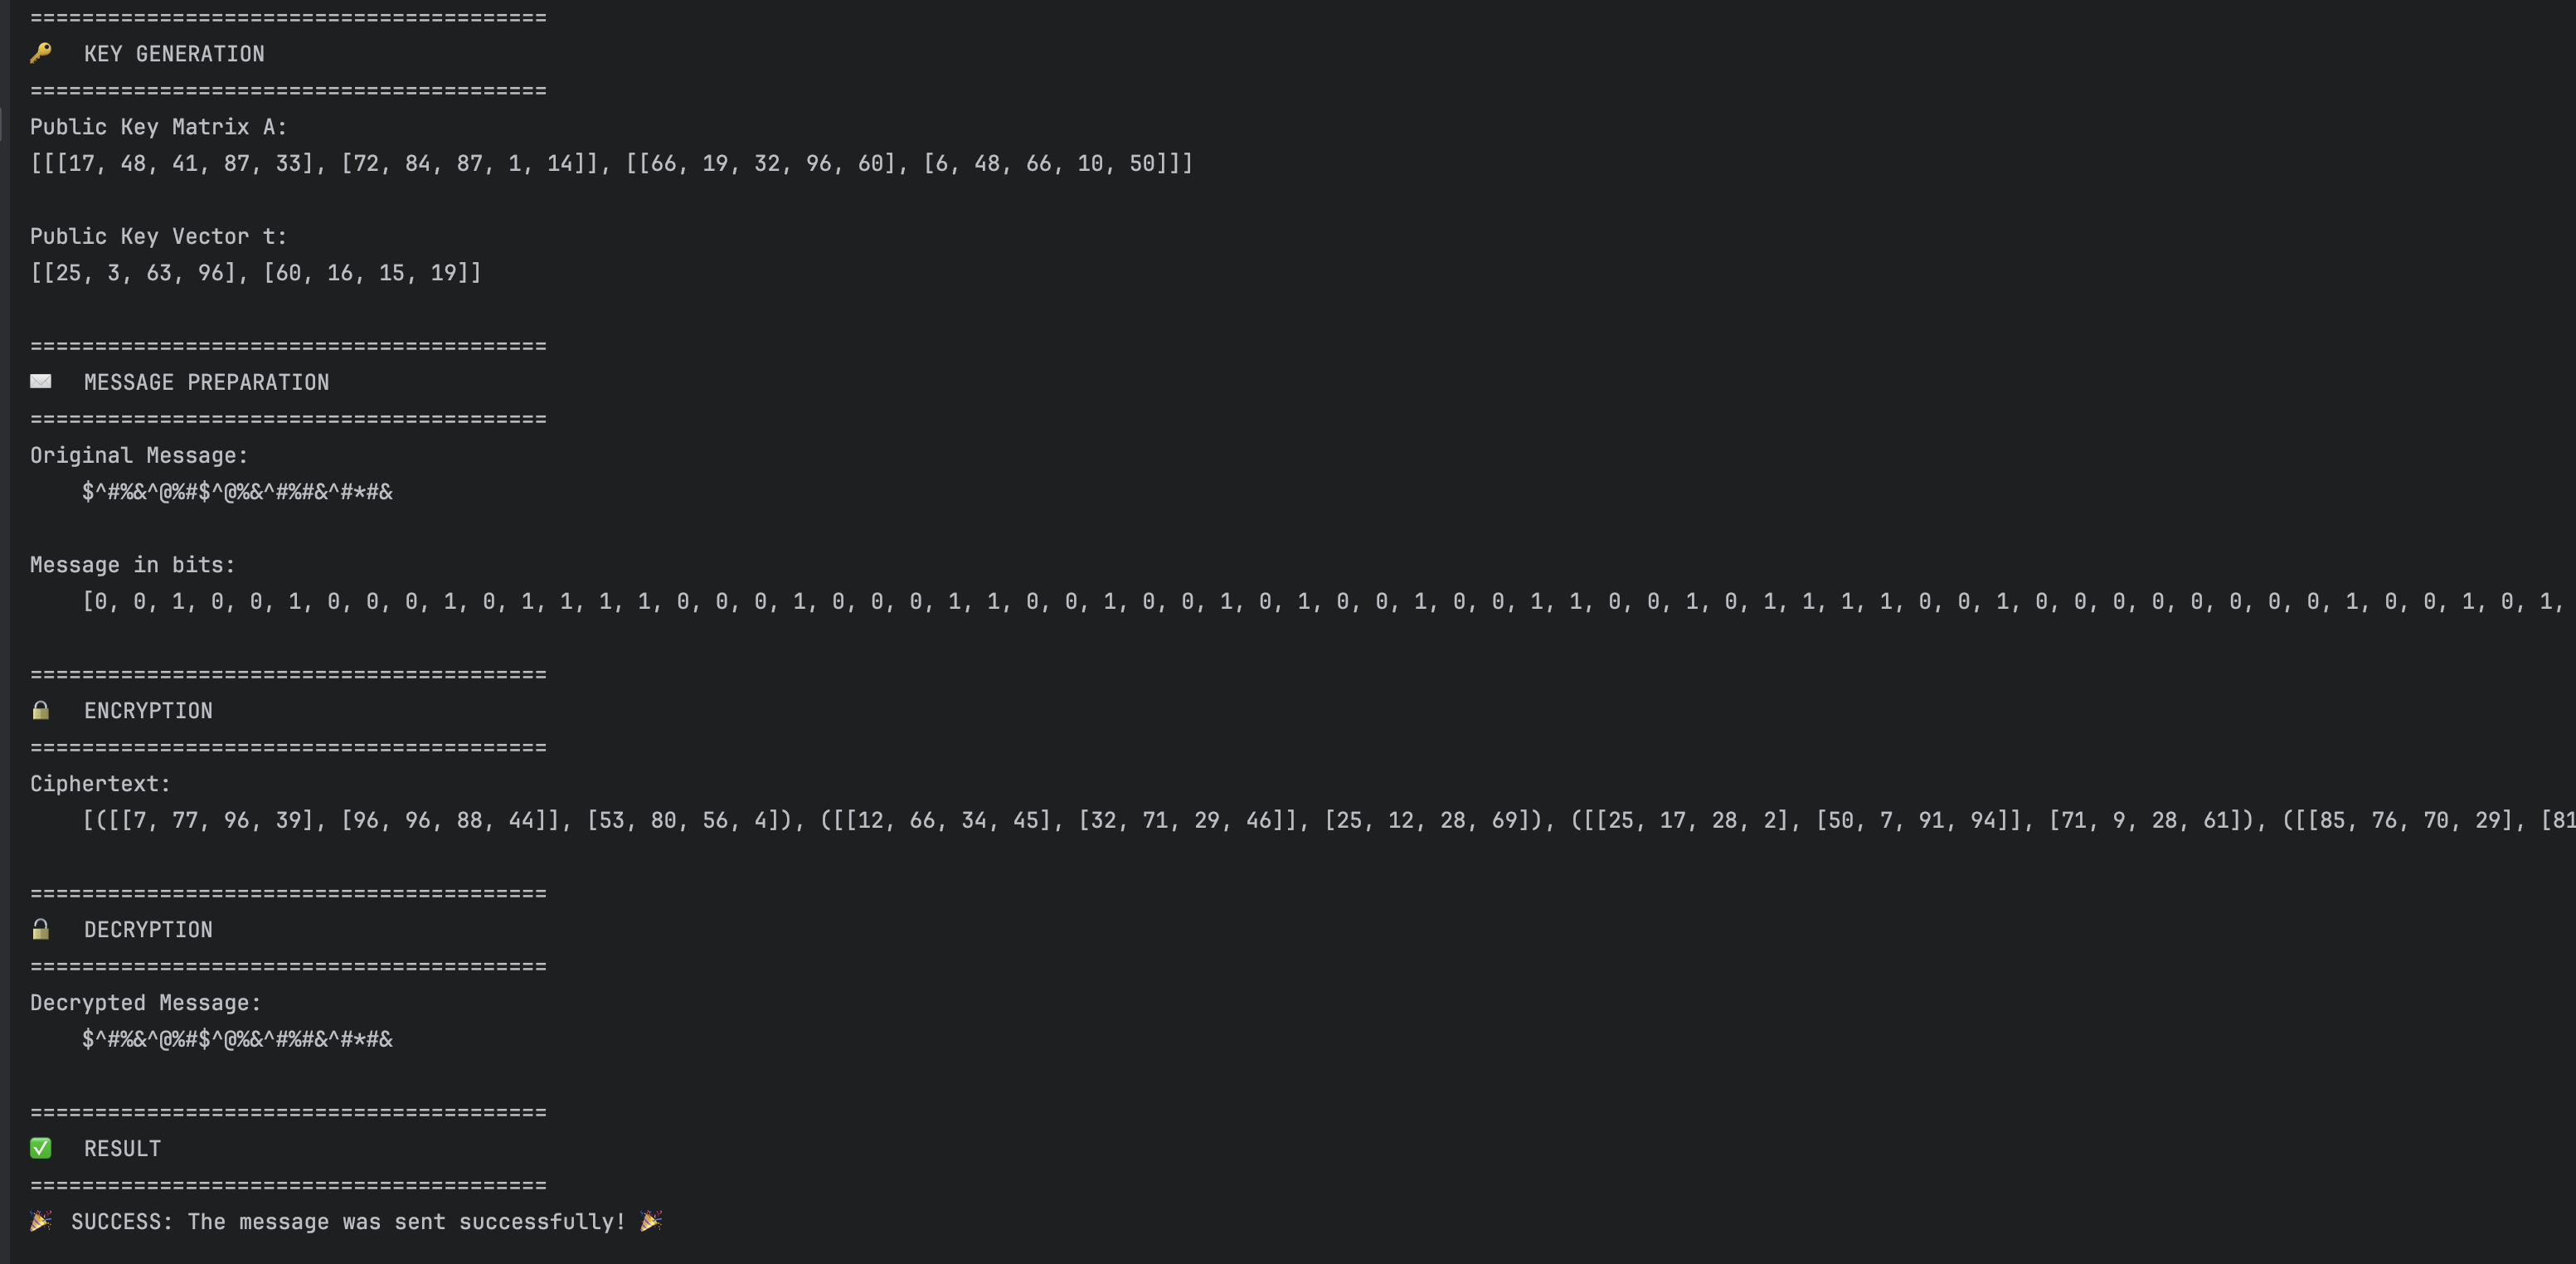
\includegraphics[width=\textwidth]{ПРАКТИКА/Images/test_4.png}
    \caption{Результат 4}
\end{figure}

\begin{figure}[h]
    \centering
    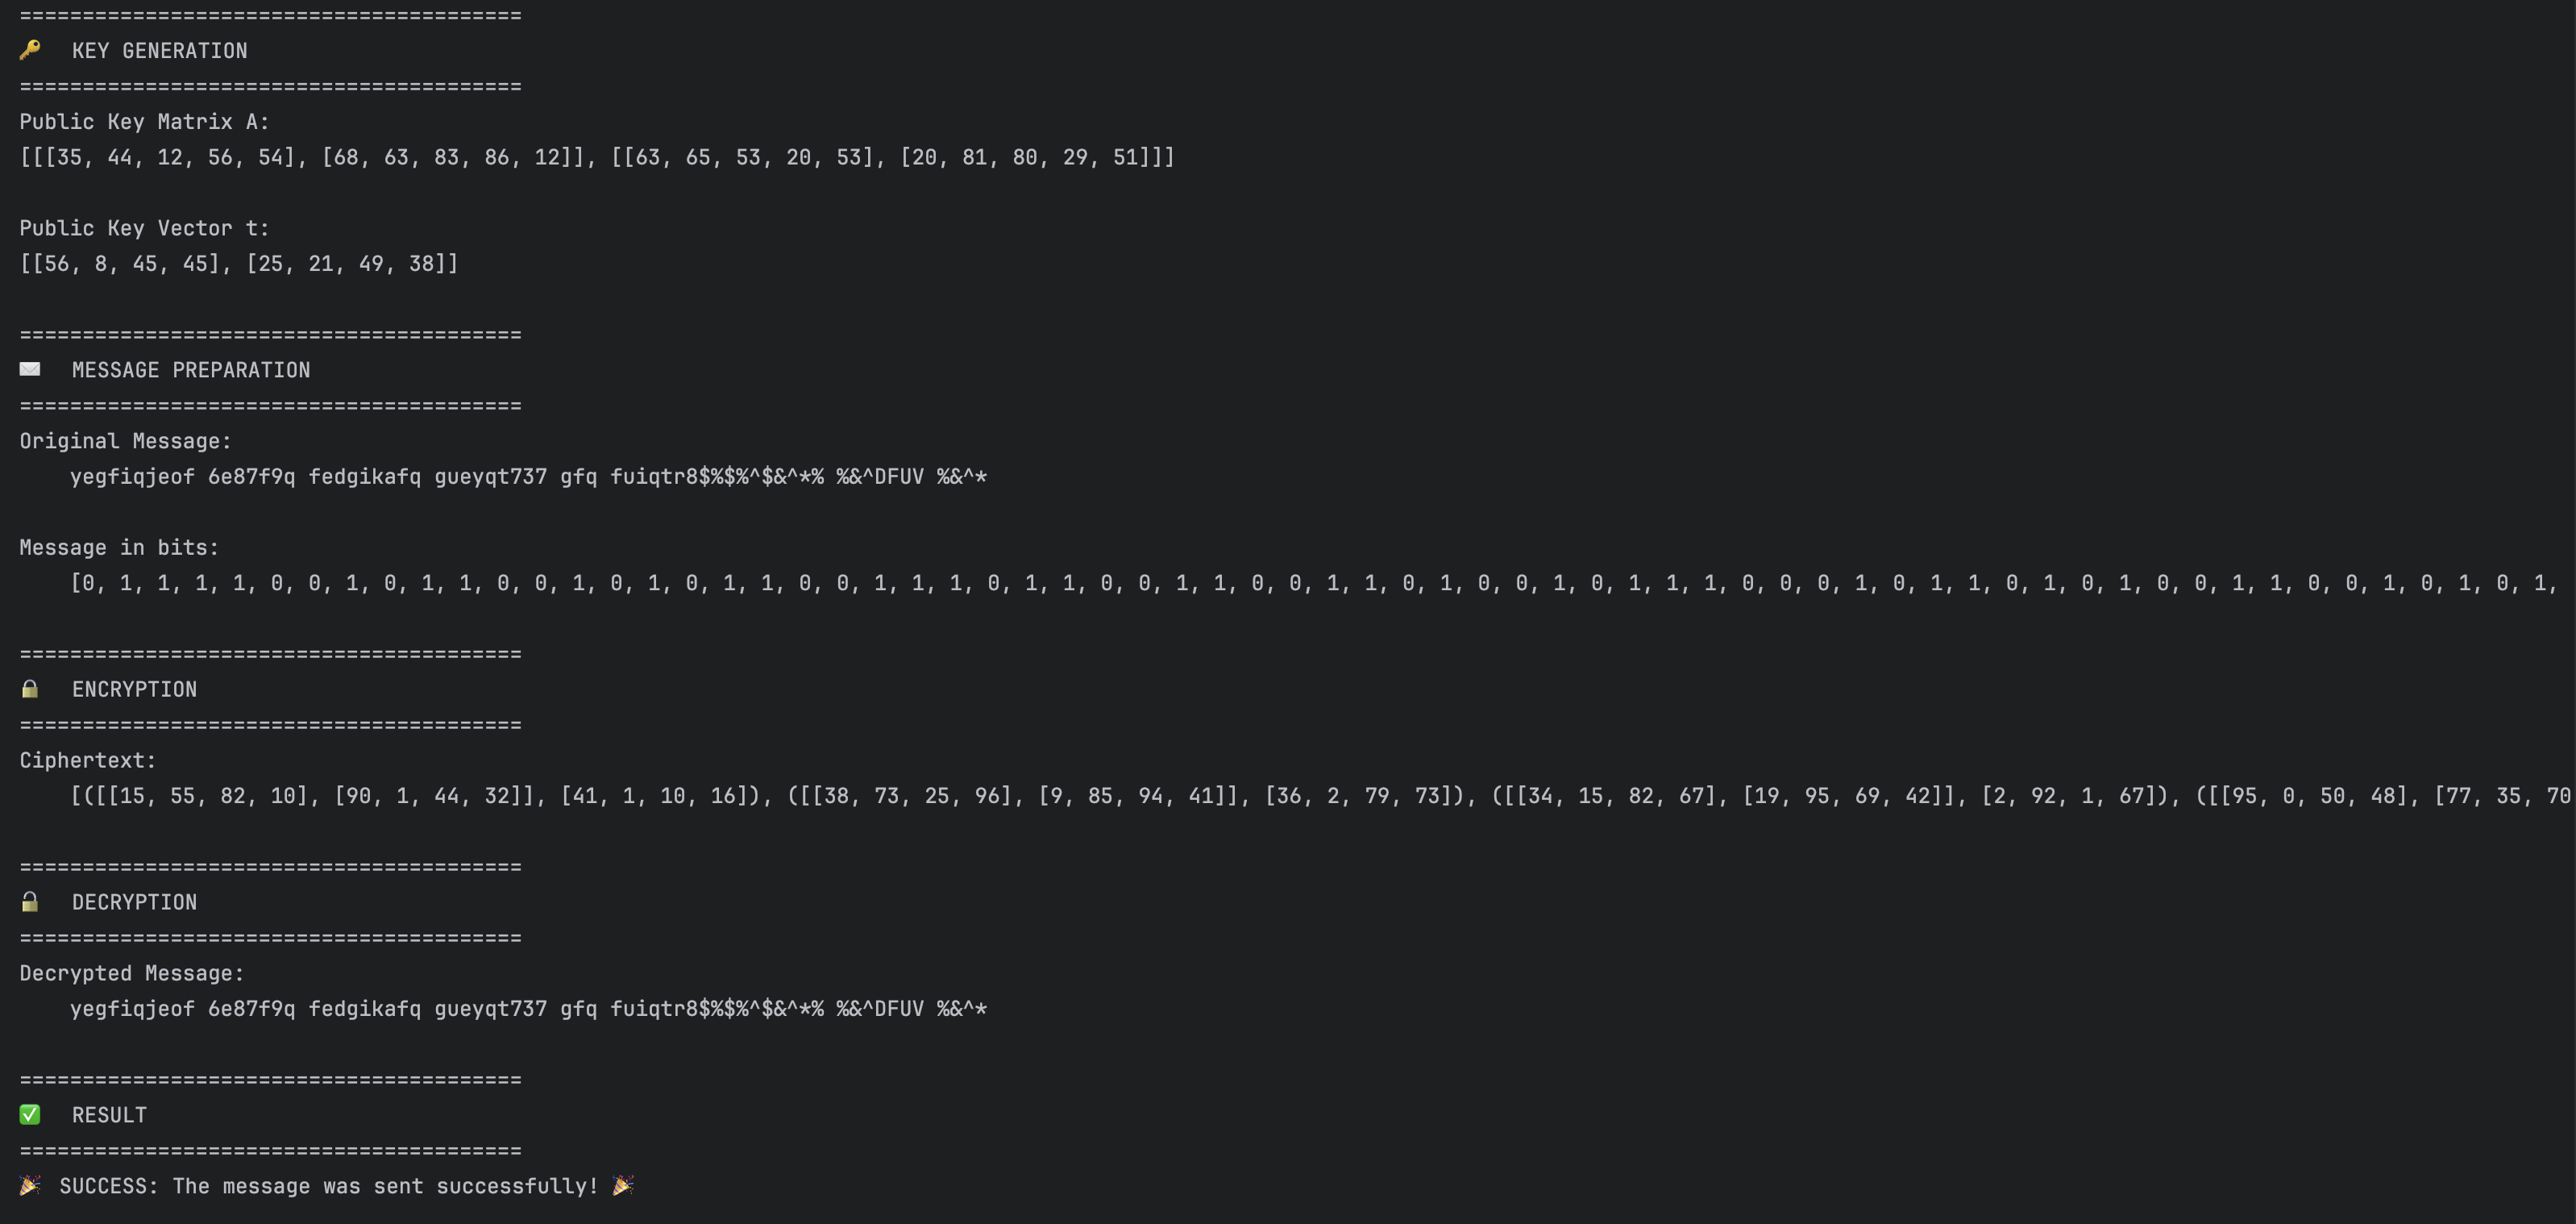
\includegraphics[width=\textwidth]{ПРАКТИКА/Images/test_5.png}
    \caption{Результат 5}
\end{figure}
%!TEX root = ../thesis.tex
% створюємо розділ
\chapter{Оцінка стійкості реалізованої конструкції до вимог IND-CPA та IND-CCA}
\label{chap:chapter2}  

У цьому розділі буде здійснено аналіз відповідності реалізованої криптографічної конструкції вимогам двох основних моделей безпеки: IND-CPA та IND-CCA. Перш за все, розглянемо теоретичні основи цих моделей безпеки, щоб зрозуміти, як вони визначають рівень стійкості криптографічних схем. Далі буде проведена оцінка стійкості конструкції до цих вимог, а також порівняння стійкості конструкції до кожної з моделей. Завершальний етап включатиме практичну реалізацію атак, які дозволять перевірити, наскільки добре конструкція Baby Kyber витримує загрози згідно з обраними моделями безпеки.

%%% --------------------------------------------------------
\section{Вступ до моделей безпеки IND-CPA та IND-CCA}
%%% --------------------------------------------------------

\subsection*{IND-CPA стійкість}
 Безпека є найважливішою складовою будь-якої схеми і її забезпечення є головною задачею дослідника. Звичайне поняття безпеки дуже схоже на концепцію безпеки шифрування з відкритим ключем. Основною ідеєю є те, що зловмисник не повинен мати змогу визначити, чи міститься конкретний ключ в зашифрованому тексті. Інакше кажучи, зловмисник не повинен відрізнити випадковий ключ від ключа, який був зашифрований~\cite{KEMProof}. 

 Механізм інкапсуляції ключів вважається стійким до атаки обраним відкритим текстом (IND-CPA), якщо зловмисник $\mathcal{A}$ не може відрізнити спільний ключ від випадкового спільного ключа з імовірністю більше, ніж~$\frac{1}{2}$. Зловмисник $\mathcal{A}$ отримує всю відкриту інформацію, яка створена КЕМ. Це визначення параметризується розподілом S, який описує безпечне джерело спільних секретів. Варто зазначити, що КЕМ не має відкритого тексту, проте це поняття використовується у визначенні через аналогію з відповідними поняттями у шифруванні~\cite{Campagna2020}. 

Для доведення IND-CPA стійкості будують так звані IND-CPA ігри: 
\begin{figure}[h]
    \centering
    \renewcommand{\arraystretch}{1.5}
    \setlength{\tabcolsep}{6pt}
    
    \begin{tabular}{|c|}
        \hline
        \textbf{Game} $G0_{KEM}^{ind-cpa}(\mathcal{A})$ \\
        \hline
        $(\cdot, P) \gets_{\$} \textbf{KGen}()$ \\
        $(k, R) \gets_{\$} \textbf{Enc}(P)$ \\
        $\textbf{if } \perp(k, R) \textbf{ return } 0$ \\
        $\textbf{return } \mathcal{A}(P, R, k)$ \\
        \hline
    \end{tabular}
    \hspace{0.5cm}
    \begin{tabular}{|c|}
        \hline
        \textbf{Game} $G1_{KEM, S}^{ind-cpa}(\mathcal{A})$ \\
        \hline
        $(\cdot, P) \gets_{\$} \textbf{KGen}()$ \\
        $(k, R) \gets_{\$} \textbf{Enc}(P), k' \gets_{\$} \textbf{S}()$ \\
        $\textbf{if } \perp(k, R) \textbf{ return } 0$ \\
        $\textbf{return } \mathcal{A}(P, R, k')$ \\
        \hline
    \end{tabular}
    
    \caption{IND-CPA ігри}
\end{figure}

\begin{definition}~\cite{Campagna2020} (IND-CPA перевага)
    Нехай КЕМ --- механізм інкапсуляції ключів, $\mathcal{A}$ - алгоритм. Тоді, перевага $\mathcal{A}$ над IND-CPA KEM джерела S дорівнює: 
    $$Adv_{KEM, S}^{ind-cpa}(\mathcal{A}) = |Pr[G0_{KEM}^{ind-cpa}(\mathcal{A}) = 1] - Pr[G1_{KEM, S}^{ind-cpa}(\mathcal{A}) = 1] |$$
\end{definition}


\subsection*{IND-CCA стійкість}
 Існує і більш сильний варіант захисту. Тут зловмисник може робити запити на розшифрування вибраних ним зашифрованих текстів. Такі атаки називаються атаками на основі обраних шифротекстів (ССА). Вони моделюють ситуацію, у яких можливе знання ключів, що містяться в певних зашифрованих текстах. Хоча на практиці такі витоки зазвичай обмежені, більш загальна модель безпеки враховує ширший спектр загроз, що дозволяє побудувати схеми, які задовольняють загальну модель~\cite{KEMProof}. 

Насправді, концепція цієї атаки ідентична із IND-CPA за винятком того, що зловмисник також має змогу здійснити атаку за допомогою обраного шифротексту, адже має доступ до оракула декапсуляції. Він може викликати такий оракул для будь-яких шифротекстів, окрім тих які безпосередньо беруть участь у грі~\cite{Campagna2020}. 

Для доведення IND-CCA стійкості будують так звані IND-CCA ігри~\cite{Campagna2020}:
\begin{figure}[h]
    \centering
    \renewcommand{\arraystretch}{1.5}
    \setlength{\tabcolsep}{6pt}
    
    \begin{tabular}{|c|}
        \hline
        \textbf{Game} $G0^{ind-cca}_{KEM}(\mathcal{A})$ \\
        \hline
        $(sk, pk) \gets_{\$} \textbf{KGen}()$ \\
        $(k, c) \gets_{\$} \textbf{Enc}(pk)$ \\
        $\textbf{if } \perp(k) \textbf{ return } 0$ \\
        $\textbf{return } \mathcal{A}^{\mathcal{D}^{sk, c}}(pk, c, k)$ \\
        \hline
    \end{tabular}
    \hspace{0.5cm}
    \begin{tabular}{|c|}
        \hline
        \textbf{Game} $G1^{ind-cca}_{KEM, S}(\mathcal{A})$ \\
        \hline
        $(sk, pk) \gets_{\$} \textbf{KGen}()$ \\
        $(k, c) \gets_{\$} \textbf{Enc}(pk), k' \gets_{\$} \textbf{S}()$ \\
        $\textbf{if } \perp(k) \textbf{ return } 0$ \\
        $\textbf{return } \mathcal{A}^{\mathcal{D}^{sk, c}}(pk, c, k')$ \\
        \hline
    \end{tabular}
    
    \caption{IND-CCA games}
\end{figure}

\begin{definition}~\cite{Campagna2020} (IND-CСА перевага)
    Нехай КЕМ --- механізм інкапсуляції ключів, $\mathcal{A}$ - алгоритм зловмисника. Тоді, перевага $\mathcal{A}$ над IND-CCA KEM джерела S дорівнює: 
    $$Adv_{KEM, S}^{ind-cca}(\mathcal{A}) = |Pr[G0_{KEM}^{ind-cca}(\mathcal{A}) = 1] - Pr[G1_{KEM, S}^{ind-cca}(\mathcal{A}) = 1] |$$
\end{definition}


%%% --------------------------------------------------------
\section{Оцінка стійкості Baby Kyber до вимог IND-CPA та IND~-CCA}
%%% --------------------------------------------------------

\subsection*{Оцінка стійкості Baby Kyber до IND-CPA}

Стійкість криптографічної схеми до атаки IND-CPA є одним із важливих критеріїв її безпеки. Для оцінки цієї стійкості необхідно проаналізувати здатність зловмисника відрізнити зашифровані версії двох різних повідомлень, згенерованих за допомогою відкритого ключа, без доступу до особистого ключа. У контексті Baby Kyber, ця стійкість визначається здатністю схемі забезпечити безпечне шифрування, яке не дозволяє зловмиснику здобути корисну інформацію про повідомлення, навіть якщо він має доступ до численних зашифрованих повідомлень.

Для доведення стійкості побудуємо IND-CPA гру. Гра IND-CPA моделює атаку зловмисника, який має доступ до відкритого ключа та оракула шифрування. Мета --- перевірити, чи зможе він відрізнити, яке з двох повідомлень було зашифроване.

\textbf{1. Ініціалізація}

Оракул генерує ключі для Baby Kyber:
\begin{itemize}
    \item Випадкова матриця: $A \in \mathbb{Z}_q[X]^{k \times k} / (X^n + 1)$.
    \item Вектори $s, e \sim \text{CBD}$ --- шум, згенерований через центральний біноміальний розподіл.
    \item Обчислення: $t = A s + e$.
    \item Відкритий ключ: $pk = (A, t)$, особистий ключ: $sk = s$.
    \item Оракул передає зловмиснику $pk$.
\end{itemize}

\textbf{2. Шифрування}

Зловмисник $\mathcal{A}$ може багаторазово шифрувати повідомлення $m$:
\begin{enumerate}
    \item Надсилає $m$ до оракула.
    \item Оракул:
    \begin{itemize}
        \item Вибирає $r, e_1, e_2 \sim \text{CBD}$.
        \item Обчислює шифротекст:
        \[
        u = A^T r + e_1,\quad v = t^T r + e_2 + \left\lfloor \frac{q}{2} \right\rfloor m.
        \]
        \item Повертає $c = (u, v)$.
    \end{itemize}
\end{enumerate}

\textbf{3. Вибір повідомлень (Challenge Phase)}

\begin{itemize}
    \item Супротивник обирає два повідомлення $m_0, m_1$ однакової довжини.
    \item Надсилає $(m_0, m_1)$ оракулу.
    \item Оракул вибирає випадковий біт $b \in \{0, 1\}$ та нові випадкові $r^*, e_1^*, e_2^*$.
    \item Обчислює:
    \[
    u^* = A^T r^* + e_1^*,\quad v^* = t^T r^* + e_2^* + \left\lfloor \frac{q}{2} \right\rfloor m_b.
    \]
    \item Повертає $c^* = (u^*, v^*)$ супротивнику.
\end{itemize}

\textbf{4. Вгадування}

\begin{itemize}
    \item Супротивник аналізує $c^*$ та видає здогад $b' \in \{0, 1\}$.
    \item Якщо $b' = b$, то супротивник виграв гру.
\end{itemize}


\begin{figure}[h]
    \centering
    \renewcommand{\arraystretch}{1.5}
    \setlength{\tabcolsep}{6pt}
    
    \begin{tabular}{|c|}
        \hline
        \textbf{Game} $G_0^{\mathsf{ind\text{-}cpa}}(\mathcal{A})$ \\
        \hline
        $(s, e) \gets_{\$} \text{CBD}$ \\
        $A \gets_{\$} \mathbb{Z}_q[X]^{k \times k} / (X^n + 1)$ \\
        $t = A s + e$ \\
        $pk = (A, t),\quad sk = s$ \\
        $\mathcal{A}$ receives $pk$ and access to $\mathsf{Enc}(\cdot)$ \\
        $(m_0, m_1) \gets \mathcal{A}$ \\
        $b \gets_{\$} \{0,1\}$ \\
        $r, e_1, e_2 \gets_{\$} \text{CBD}$ \\
        $u = A^T r + e_1$ \\
        $v = t^T r + e_2 + \left\lfloor \frac{q}{2} \right\rfloor m_b$ \\
        $c^* = (u, v)$ \\
        $b' \gets \mathcal{A}(c^*)$ \\
        \textbf{return} $[b' = b]$ \\
        \hline
    \end{tabular}
    
    \caption{IND-CPA гра для Baby Kyber}
\end{figure}

\newpage
Щоб з'ясувати, чи може зловмисник визначити біт $b$, розглянемо, наскільки компоненти шифротексту $u$ та $v$ приховують інформацію про повідомлення $m_b$.

\textbf{Розподіл $u$}

Шифротекст $u$ визначається як:
\[
u = A^T r + e_1
\]
\begin{itemize}
    \item $A$ --- публічна випадкова матриця поліномів.
    \item $r \sim \text{CBD}$ --- випадковий вектор поліномів, незалежний від $A$.
    \item  $A^T r$ --- виглядає як випадковий вектор.
    \item Додавання шуму $e_1$ (також з розподілу CBD) ще більше ускладнює структуру $u$.
\end{itemize}

$u$ виглядає як повністю випадковий вектор, незалежний від $m_b$.

\textbf{Розподіл $v$}

Компонент $v$ задається як:
\[
v = t^T r + e_2 + \left\lfloor \frac{q}{2} \right\rfloor m_b
\]
Підставимо $t = A s + e$:
\[
\begin{aligned}
v &= (A s + e)^T r + e_2 + \left\lfloor \frac{q}{2} \right\rfloor m_b \\
  &= s^T (A^T r) + e^T r + e_2 + \left\lfloor \frac{q}{2} \right\rfloor m_b
\end{aligned}
\]

\begin{itemize}
    \item $s$ --- секретний вектор, недоступний для супротивника.
    \item $A^T r$ --- випадковий вектор, незалежний від $s$.
    \item Добуток $s^T (A^T r)$ має вигляд випадкового полінома.
    \item Шум $e^T r + e_2$ ще більше маскує значення.
\end{itemize}

$v$ також виглядає як випадковий елемент, і $m_b$ у ньому не видимий через шум.


IND-CPA-стійкість означає, що зловмисник не може відрізнити, яке з двох повідомлень $m_0, m_1$ було зашифроване, навіть маючи доступ до:
\begin{itemize}
    \item Публічного ключа $pk = (A, t)$.
    \item Оракула шифрування: $\mathsf{Encrypt}(pk, \cdot)$.
    \item Шифротексту $c^* = (u, v)$, що містить зашифроване $m_b$.
\end{itemize}

Схема є IND-CPA стійкою тому що: 
\begin{itemize}
    \item Рандомізація через $r$ гарантує, що одне й те саме повідомлення шифрується кожного разу інакше.
    \item Шумові доданки $e_1$, $e_2$ та $e$ приховують структуру повідомлення.
    \item Без знання $s$ неможливо відновити $m_b$ з $v$.
    \item Побудовано на задачі Learning With Errors (LWE), яка вважається складною навіть для квантових обчислень.
\end{itemize}

Інформація про $m_b$ не витікає із шифротексту, тому схема є стійкою до IND-CPA атак.


\subsection*{Оцінка стійкості Baby Kyber до IND-CCA}

Стійкість криптографічної схеми до атаки IND-CCA є більш суворим критерієм безпеки, ніж стійкість до IND-CPA. У цьому випадку зловмисник може не лише отримати зашифровані повідомлення, а й зробити запити на дешифрування обраних шифротекстів, що дає йому додаткову інформацію, яку можна використати для атаки на схему. Оцінка стійкості Baby Kyber до IND-CCA ґрунтується на здатності схеми зберігати конфіденційність повідомлення навіть при наявності такого доступу до шифротекстів.

Для доведення стійкості побудуємо IND-CСA гру. Гра IND-CСA моделює атаку зловмисника, який має доступ до відкритого ключа, оракула шифрування та оракула дешифрування. Мета --- перевірити, чи зможе він відрізнити, яке з двох повідомлень було зашифроване.

\textbf{1. Ініціалізація}

Оракул генерує ключі для Baby Kyber:

– Випадкова матриця:  
\[
A \in \mathbb{Z}_q[X]^{k \times k} / (X^n + 1)
\]

– Вектори $s, e \sim \text{CBD}$ — шум, згенерований через центрований біноміальний розподіл.

– Обчислення:
\[
t = As + e
\]

– Відкритий ключ: $pk = (A, t)$, особистий ключ: $sk = s$.

– Оракул передає зловмиснику $pk$.

– Також зловмиснику надається доступ до оракула дешифрування: $\mathcal{D}(c) = \mathsf{Dec}_{sk}(c)$, з обмеженням, що не можна подавати $c = c^*$ у фазі виклику.

\textbf{2. Шифрування}

Зловмисник $\mathcal{A}$ може багаторазово шифрувати повідомлення $m$:

1) Надсилає $m$ до оракула.

2) Оракул:

– Вибирає $r, e_1, e_2 \sim \text{CBD}$.

– Обчислює шифротекст:
\[
u = A^T r + e_1, \quad v = t^T r + e_2 + \left\lfloor \frac{q}{2} \right\rfloor m
\]

– Повертає $c = (u, v)$.

– Зловмисник може також надсилати запити на дешифрування довільних $c \ne c^*$, використовуючи оракул $\mathcal{D}$.

\textbf{3. Вибір повідомлень (Challenge Phase)}

– Зловмисник обирає два повідомлення $m_0, m_1$ однакової довжини.

– Надсилає $(m_0, m_1)$ оракулу.

– Оракул вибирає випадковий біт $b \in \{0,1\}$ та нові випадкові значення $r^*, e_1^*, e_2^*$.

– Обчислює:
\[
u^* = A^T r^* + e_1^*, \quad v^* = t^T r^* + e_2^* + \left\lfloor \frac{q}{2} \right\rfloor m_b
\]

– Повертає $c^* = (u^*, v^*)$ зловмиснику.

– Забороняє надсилати $c^*$ до оракула дешифрування.

\textbf{4. Вгадування}

– Зловмисник аналізує $c^*$, продовжує робити дозволені запити до оракула дешифрування $\mathcal{D}(c \ne c^*)$.

– Видає здогад $b' \in \{0, 1\}$.

– Якщо $b' = b$, то зловмисник виграв гру.


\begin{figure}[h]
    \centering
    \renewcommand{\arraystretch}{1.6}
    \setlength{\tabcolsep}{8pt}

    \begin{tabular}{|p{7.1cm}|p{6.7cm}|}
        \hline
        \multicolumn{2}{|c|}{\textbf{Game} $G_0^{\mathsf{ind\text{-}cca}}(\mathcal{A})$} \\
        \hline
        $(s, e) \gets_{\$} \text{CBD}$ & $A \gets_{\$} \mathbb{Z}_q[X]^{k \times k} / (X^n + 1)$ \\
        $t = As + e$ & $pk = (A, t),\quad sk = s$ \\
        \textit{$\mathcal{A}$ receives $pk$, access to $\mathsf{Enc}(\cdot)$ and $\mathsf{Dec}(\cdot \ne c^*)$} & \\
        $(m_0, m_1) \gets \mathcal{A},\quad b \gets_{\$} \{0,1\}$ & \\
        $r^*, e_1^*, e_2^* \gets_{\$} \text{CBD}$ & $u^* = A^T r^* + e_1^*$ \\
        $v^* = t^T r^* + e_2^* + \left\lfloor \frac{q}{2} \right\rfloor m_b$ & $c^* = (u^*, v^*)$ \\
        \textit{$\mathcal{A}$ may query $\mathsf{Dec}(c)$ for $c \ne c^*$} & \\
        $b' \gets \mathcal{A}(c^*)$ & \\
        \multicolumn{2}{|c|}{\textbf{return} $[b' = b]$} \\
        \hline
    \end{tabular}

    \caption{IND-CCA гра для Baby Kyber}
\end{figure}


Щоб з’ясувати, чи може зловмисник визначити біт $b$, розглянемо, наскільки компоненти шифротексту $u$ та $v$ приховують інформацію про повідомлення $m_b$, якщо зловмисник має доступ до оракула дешифрування.

\textbf{Модель атаки}

У моделі IND-CCA зловмисник має доступ до:

\begin{itemize}
    \item Публічного ключа $pk = (A, t)$
    \item Оракула шифрування: $\mathsf{Enc}(pk, \cdot)$
    \item Оракула дешифрування: $\mathsf{Dec}(sk, \cdot)$, з обмеженням $c \ne c^*$
\end{itemize}

Задача зловмисника — вгадати біт $b$ за шифротекстом $c^* = (u^*, v^*)$, який є шифруванням одного з повідомлень $m_0, m_1$.

\textbf{Вразливість шифротексту}

Challenge-шифротекст має вигляд:
\[
c^* = (u^*, v^*) = (A^T r^* + e_1^*,\quad t^T r^* + e_2^* + \left\lfloor \frac{q}{2} \right\rfloor m_b)
\]

Супротивник може сконструювати змінений шифротекст:
\[
c' = (u^*, v^* + \delta)
\]
і передати його на дешифрування. Якщо $m_b = 1$, $v^*$ має зсув $\left\lfloor \frac{q}{2} \right\rfloor$, якщо $m_b = 0$ — ні.

Проаналізувавши результат розшифрування $c'$, зловмисник може зробити висновок про значення $m_b$.

\textbf{Відсутність цілісності}

Схема Baby Kyber не містить механізму перевірки автентичності:

\begin{itemize}
    \item Немає хеш-функцій або автентифікаторів у шифротексті
    \item Немає симетричної перевірки чи зв’язування $u$ і $v$
    \item Шум $e_1$, $e_2$ не гарантує безпеку від модифікації
\end{itemize}

Це дозволяє зловмиснику модифікувати $v^*$ та отримувати детерміновану зміну результату дешифрування.

Отже, зловмисник може розшифрувати змінений шифротекст $c'$ на основі $c^*$. А результат дешифрування допомагає вивести біт $b$. Саме тому схема не є IND-CCA стійкою.



\subsection*{Порівняння стійкості до IND-CPA та IND-CCA}

\begin{table}[h]
    \centering
    \renewcommand{\arraystretch}{1.6}
    \setlength{\tabcolsep}{10pt}
    \caption{Порівняння стійкості Baby Kyber до IND-CPA та IND-CCA}
    \begin{tabular}{|p{5.3cm}|p{4.5cm}|p{4.5cm}|}
        \hline
        \textbf{Критерій} & \textbf{IND-CPA} & \textbf{IND-CCA} \\
        \hline
        Модель зловмисника & Має доступ до шифрування (Enc), може надсилати будь-які повідомлення & Має доступ до шифрування (Enc) і дешифрування (Dec), крім $c^*$ \\
        \hline
        Доступ до дешифрування & Відсутній & Дозволено, але $c \ne c^*$ \\
        \hline
        Тип атаки & Вибір відкритого тексту (Chosen Plaintext) & Вибір шифротексту (Chosen Ciphertext) \\
        \hline
        Стійкість Baby Kyber & Стійкий & Не стійкий \\
        \hline
        Причини стійкості / нестійкості & Випадковість $r$, шум $e_1, e_2$ та структура $v$ приховують $m_b$ & Можна модифікувати $v^*$ і проаналізувати відповідь дешифрування \\
        \hline
        Приховування $m_b$ & Ефективне через шум і LWE & Частково порушується через можливість змінювати $v$ \\
        \hline
        Перевірка цілісності шифротексту &  Відсутня, але не критично &  Відсутня, що робить можливими атаки \\
        \hline
        Основна уразливість & — & Challenge можна змінити, зловмисник аналізує результат \\
        \hline
        Захист від модифікації $c^*$ & — &  Відсутній \\
        \hline
        Рівень безпеки & Семантична безпека при шифруванні & Семантична безпека + автентичність \\
        \hline
    \end{tabular}
\end{table}

Проведене порівняння показує, що Baby Kyber є надійною схемою шифрування з відкритим ключем у моделі IND-CPA, але не забезпечує захисту від IND-CCA атак.

У моделі IND-CPA зловмисник обмежений лише доступом до шифрування. У такому середовищі Baby Kyber демонструє високу стійкість завдяки використанню:
\begin{itemize}
    \item випадкових векторів при шифруванні;
    \item шумових членів, що маскують повідомлення;
    \item математичної складності задачі Learning With Errors (LWE).
\end{itemize}

Однак у моделі IND-CCA, де зловмисник також має доступ до оракула дешифрування, виявляється серйозна вразливість. Через відсутність перевірки цілісності шифротексту, зловмисник може модифікувати частину challenge-шифротексту (наприклад, компонент $v^*$) і використовувати оракул дешифрування для витоку інформації про зашифроване повідомлення. Це робить Baby Kyber нестійким до IND-CCA атак у базовій формі.


%%% --------------------------------------------------------
\section{Практична реалізація атак на відповідність моделям IND-CPA та IND-CCA}
%%% --------------------------------------------------------

У цьому підрозділі буде розглянуто практичну реалізацію атак IND-CPA та IND-CCA на спрощену версію Baby Kyber.  Буде подано опис основних компонентів атак, включаючи побудову викликів з боку супротивника, моделювання доступу до оракула шифрування та аналіз виграшу. Завершальною частиною стане перевірка коректності реалізації та оцінка ймовірності успішної атаки відповідно до теоретичних моделей IND-CPA та IND-CCA, описаних вище.

\subsection*{Реалізація атаки для IND-CPA}

З метою оцінки стійкості реалізованої спрощеної версії Baby Kyber до IND-CPA-атак, було проведено експеримент, в якому моделюється поведінка зловмисника з доступом до оракула шифрування.

Для реалізації атаки було створено адаптивну стратегію, за якою зловмисник:

\begin{enumerate}
    \item Ініціалізує параметри криптосистеми: розмір кільця $n$, модуль $q$, параметри шуму $\eta$ тощо, та генерує відкритий ключ $(A, t)$ і особистий ключ~$s$.
    
    \item Обирає два повідомлення $m_0$ і $m_1$, які представлені векторами з нулів та одиниць відповідно.
    
    \item Отримує шифротексти для обох повідомлень — $c_0$ та $c_1$, — та обчислює їхні оцінки, що ґрунтуються на сумі перших коефіцієнтів шифротекстів $u[0][0]$ та $v[0]$.
    
    \item Отримує шифротекст виклику $c^\star$ на одному з повідомлень $m_b$, де біт $b$ обирається випадковим чином.
    
    \item Порівнює оцінку $c^\star$ з оцінками $c_0$ та $c_1$ та вгадує, яке з повідомлень було зашифровано. Якщо відстань до $c_0$ менша — зловмисник вгадує $b=0$, інакше — $b=1$.
    
    \item Підраховує кількість успішних вгадувань за велику кількість запусків та оцінює статистичну значущість результатів.
\end{enumerate}

Результати експерименту виводяться у вигляді:
\begin{itemize}
    \item Кількості вдалих вгадувань правильного повідомлення;
    \item Ймовірності успішного вгадування;
    \item Виграшу зловмисника порівняно з випадковим вгадуванням;
    \item p-значення (p-value), що вказує на статистичну значущість результатів;
    \item 95\% довірчого інтервалу.
\end{itemize}

Для перевірки гіпотези про те, що зловмисник діє не краще за випадкове вгадування, було використано біноміальний тест із пакету \texttt{scipy.stats}. Статистичний аналіз дозволяє зробити висновки про вразливість реалізації до IND-CPA атак.

\textbf{Результати тестування:} нижче детально описані результати атаки, зображені на рисунку~\ref{fig:ind_cpa_1}.

\begin{itemize}
    \item Adversary success rate = 4971/10000
    \item Probability of guessing correctly =  $0.4971$: значення $0.4971$ для ймовірності успішного вгадування майже дорівнює $0.5$ — як випадкове вгадування.
    \item Advantage over random guessing = $0.0029$: перевага над випадковим вгадуванням advantage становить лише $0.0029$, тобто дуже мала.
    \item p-value (binomial test) =  $0.5687$: p-value більше за $0.05$, а отже ми не можемо відхилити нульову гіпотезу про те, що результат досягнутий випадково.
    \item 95\% confidence interval $[0.4873,\ 0.5069]$ : довірчий інтервал містить значення $0.5$, що підтверджує: статистично результат не є підозрілим.
\end{itemize}

Результати виконання атаки зображені на наступних рисунках : 

\begin{figure}[h]
    \centering
    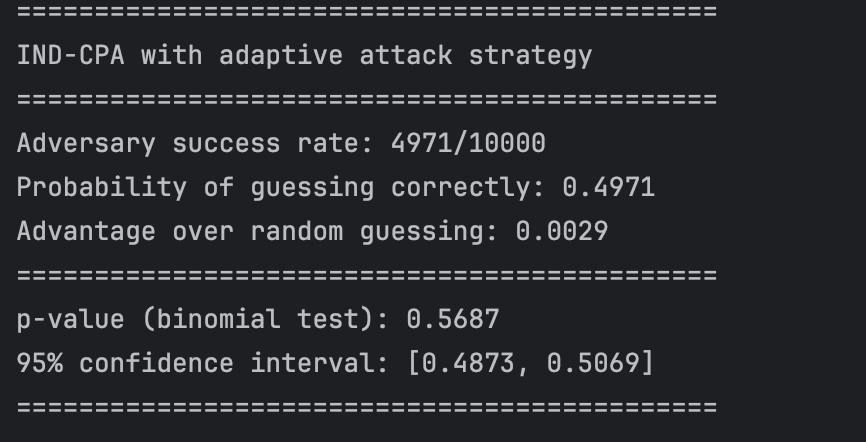
\includegraphics[width=0.925\textwidth]{ПРАКТИКА/Images/IND_CPA_1.jpg}
    \caption{Результат атаки 1}
    \label{fig:ind_cpa_1}
\end{figure}

\begin{figure}[h]
    \centering
    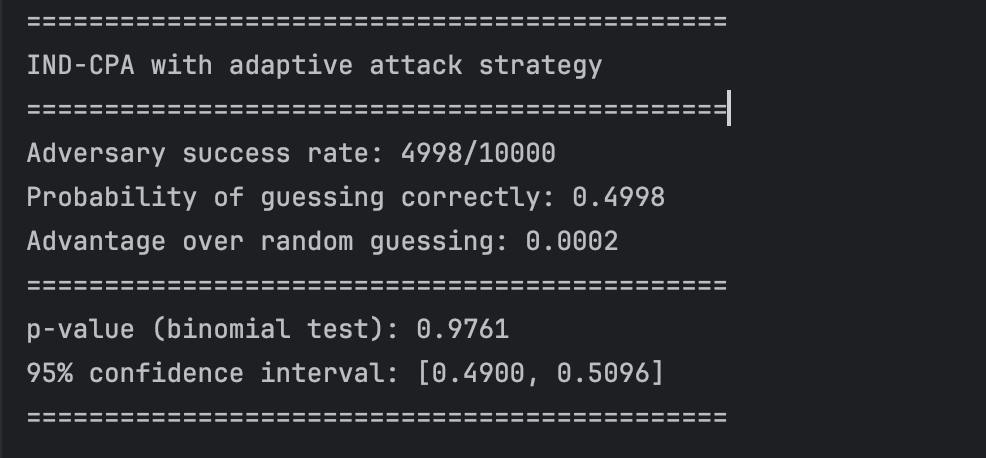
\includegraphics[width=0.925\textwidth]{ПРАКТИКА/Images/IND_CPA_2.jpg}
    \caption{Результат атаки 2}
    \label{fig:ind_cpa_2}
\end{figure}

На основі наведених результатів можна зробити висновок, що реалізований алгоритм Baby Kyber пройшов тест на стійкість до IND-CPA атаки. Успішність атакувальника статистично не відрізняється від випадкового вгадування, отже, шифрування є стійким у цій моделі безпеки.

\subsection*{Реалізація атаки для IND-CCA}

Для оцінки стійкості реалізованої версії Baby Kyber до IND-CCA - атаки було реалізовано експеримент, який моделює зловмисника, що має обмежений доступ до оракула розшифрування — без можливості розшифровувати виклик (challenge ciphertext) $c^\star$.

Атака ґрунтується на модифікації виклику $c^\star$ та аналізі результату розшифрування модифікованого шифротексту. Загальна стратегія виглядає так:

\begin{enumerate}
    \item Ініціалізується схема Baby Kyber з параметрами $q$, $n$, $k$, $\eta$. Генеруються ключі: матриця $A$, вектор $t$ та секретний ключ $s$.

    \item Зловмисник обирає два повідомлення $m_0 = [0, 0, \dots, 0]$ та $m_1 = [1, 1, \dots, 1]$, та отримує шифротекст $c^\star$ для одного з них ($m_b$), де біт $b$ обирається випадково.

    \item Створюється оракул розшифрування $D(\cdot)$, який відмовляється обробляти запити на $c^\star$, але дозволяє всі інші.

    \item Зловмисник модифікує компоненту $v^\star$ шифротексту $c^\star$, додаючи до неї невеликий відомий зсув, отримуючи змінений шифротекст $c'$.

    \item Модифікований шифротекст $c'$ передається до оракула $D(\cdot)$, який повертає розшифроване повідомлення.

    \item Якщо сума елементів у результаті розшифрування ближча до $[1, 1, \dots, 1]$, то зловмисник вгадує, що було зашифровано $m_1$, інакше — $m_0$.

    \item Після $N$ повторень експерименту обчислюються статистичні показники атаки.
\end{enumerate}

Оцінка результатів включає:

\begin{itemize}
    \item Загальну кількість вдалих вгадувань бітів $b$.
    \item Імовірність правильного вгадування ($\hat{p}$).
    \item Виграш зловмисника відносно випадкового вгадування ($|\hat{p} - 0.5|$).
    \item p-значення біноміального тесту, що оцінює статистичну значущість результату.
    \item 95\% довірчий інтервал для $\hat{p}$.
\end{itemize}

Атака демонструє можливість відхилення від ідеальної IND-CCA стійкості за рахунок експлуатації навіть мінімальних змін у шифротексті. 

\textbf{Результати тестування:} нижче детально описані результати атаки, зображені на рисунку~\ref{fig:ind_cca_1}.

\begin{itemize}
    \item Adversary success rate = 10000/10000
    \item Probability of guessing correctly = $1.0000$: ймовірність успішного вгадування становить 100\%, що свідчить про повну успішність атаки.
    \item Advantage over random guessing = $0.5000$: перевага над випадковим вгадуванням є максимальною — атакувальник завжди визначає правильне повідомлення.
    \item p-value (binomial test) = $0.0000$: надзвичайно низьке значення p-value означає, що ймовірність досягнення такого результату випадково практично нульова.
    \item 95\% confidence interval $[1.0000,\ 1.0000]$: довірчий інтервал повністю охоплює значення $1.0$, що підтверджує абсолютну впевненість у результаті.
\end{itemize}

На основі наведених результатів можна зробити висновок, що реалізований алгоритм Baby Kyber не є стійким до IND-CCA атаки. Атакувальник мав повну можливість відрізнити зашифровані повідомлення, що свідчить про критичну уразливість у цій моделі безпеки. Для забезпечення повної криптографічної стійкості необхідно впровадити відповідні механізми захисту від атак із вибраним шифротекстом.

\newpage
Результати виконання атаки зображені на рисунку:

\begin{figure}[h]
    \centering
    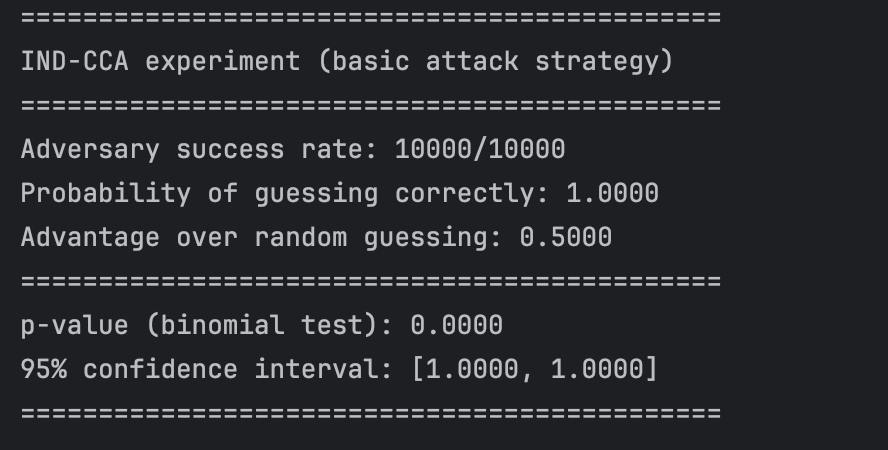
\includegraphics[width=0.925\textwidth]{ПРАКТИКА/Images/IND_CCA_1.jpg}
    \caption{Результат атаки}
    \label{fig:ind_cca_1}
\end{figure}




% Створюємо висновки
\conclusions
%!TEX root = ../thesis.tex
% створюємо Висновки до всієї роботи

У рамках переддипломної практики було реалізовано та досліджено спрощену версію постквантової криптосистеми Kyber — Baby Kyber. Було проведено теоретичний аналіз математичних основ алгоритму, визначено обмеження та особливості спрощеної моделі, зокрема фіксацію параметрів, відсутність перетворення Фур'є (NTT) та відмову від використання FO-перетворення.

Було розроблено програмну реалізацію алгоритму, яка охоплює генерацію ключів, шифрування та розшифрування повідомлень у вибраному параметричному просторі. Реалізація виконана мовою Python у середовищі PyCharm, із дотриманням модульного підходу до організації коду.

В межах експериментальної частини було проведено тестування стійкості алгоритму до атак типу IND-CPA та IND-CCA. За результатами аналізу встановлено, що реалізація демонструє статистичну стійкість до IND-CPA атак — ймовірність успішного вгадування не перевищує рівень випадковості. Водночас, алгоритм є повністю вразливим до IND-CCA атак через відсутність механізмів активного захисту, зокрема FO-перетворення.

Таким чином, реалізований алгоритм забезпечує базовий рівень конфіденційності у пасивній моделі супротивника, але не гарантує безпеки в умовах активного впливу. Робота демонструє практичне підтвердження важливості використання додаткових криптографічних трансформацій для досягнення повноцінної стійкості сучасних постквантових криптосистем.

% Додаємо бібліографію
% Якщо ви володієте магією bibtex-у, використовуйте її та модифікуйте файл 
% з бібліографією відповідним чином
%!TEX root = ../thesis.tex
% створюємо список використаної літератури
\begin{thebibliography}    
    \bibitem{KyberCCA}
       Joppe Bos, Léo Ducas and others. CRYSTALS – Kyber: a CCA-secure module-lattice-based KEM. ---  
        \newblock Cryptology ePrint Archive, Report 2017/634, 2017.  
        \newblock Режим доступу: \url{https://eprint.iacr.org/2017/634.pdf}.

    \bibitem{KyberWebsite}
        CRYSTALS-Kyber. Official website. ---  
        \newblock Режим доступу: \url{https://pq-crystals.org/kyber/}.

    \bibitem{babyKyber}
        Kyber - How does it work?: Post-Quantum Cryptography. Cryptopedia. ---  
        \newblock Режим доступу: \url{https://cryptopedia.dev/posts/kyber/}.

    \bibitem{Langlois2012}
        Langlois,~Adeline, Stehlé,~Damien. Worst-Case to Average-Case Reductions for Module Lattices. --- 
        \newblock Cryptology ePrint Archive, Paper 2012/090, 2012.  
        \newblock Режим доступу: \url{https://eprint.iacr.org/2012/090/20130815:054538}.

    \bibitem{Gonzalez2021}
        Gonzalez,~Ruben. Kyber - How does it work? ---  
        \newblock Approachable Cryptography, 2021.  
        \newblock Режим доступу: \url{https://cryptopedia.dev/posts/kyber/}.

    \bibitem{Lyubashevsky2013}
    Lyubashevsky,~Vadim, Peikert,~Chris, Regev,~Oded. On Ideal Lattices and Learning with Errors over Rings. ---  
    \newblock Journal of the ACM, vol.~60, no.~6, pp.~1--35, 2013.  
    \newblock Режим доступу: \url{https://doi.org/10.1145/2535925}.

    \bibitem{Langlois2012}
        Langlois,~Adeline, Stehlé,~Damien. Worst-Case to Average-Case Reductions for Module Lattices. ---  
        \newblock Cryptology ePrint Archive, Paper 2012/090, 2012.  
        \newblock Режим доступу: \url{https://eprint.iacr.org/2012/090/20130815:054538}.
    
    \bibitem{Pessl2017}
        Pessl,~Peter, Bruinderink,~Leon~Groot, Yarom,~Yuval. To BLISS-B or not to be - Attacking strongSwan’s Implementation of Post-Quantum Signatures. ---  
        \newblock Cryptology ePrint Archive, Paper 2017/490, 2017.  
        \newblock Режим доступу: \url{https://eprint.iacr.org/2017/490/20170828:125948}.
    
    \bibitem{Alkim2016}
        Alkim,~Erdem, Ducas,~Léo, Pöppelmann,~Thomas, Schwabe,~Peter. NewHope without reconciliation. ---  
        \newblock Cryptology ePrint Archive, Paper 2016/1157, 2016.  
        \newblock Режим доступу: \url{https://eprint.iacr.org/2016/1157/20171109:073050}.
    
    \bibitem{Avanzi2021}
        Avanzi,~Roberto, Bos,~Joppe, Ducas,~Léo, Kiltz,~Eike, Lepoint,~Tancrède, Lyubashevsky,~Vadim, Schanck,~John~M., Schwabe,~Peter, Seiler,~Gregor, Stehlé,~Damien. Algorithm Specifications and Supporting Documentation (version 3.02). ---  
        \newblock 2021.  
        \newblock Режим доступу: \url{https://pqc-hqc.org/doc/hqc-specification_2024-02-23.pdf}.
    
    \bibitem{Botros2019}
        Botros,~Leon, Kannwischer,~Matthias~J., Schwabe,~Peter. Memory-Efficient High-Speed Implementation of Kyber on Cortex-M4. ---  
        \newblock Cryptology ePrint Archive, Paper 2019/489, 2019.  
        \newblock Режим доступу: \url{https://eprint.iacr.org/2019/489/20190520:092623}.

    \bibitem{Lyubashevsky2024}
        Lyubashevsky,~Vadim. Basic Lattice Cryptography: The concepts behind Kyber (ML-KEM) and Dilithium (ML-DSA). ---  
        \newblock Cryptology ePrint Archive, Paper 2024/1287, 2024.  
        \newblock Режим доступу: \url{https://eprint.iacr.org/2024/1287/20241024:103131}.

    \bibitem{Kyber512NISTFAQ}
        FAQ on Kyber512. ---  
        \newblock National Institute of Standards and Technology (NIST).  
        \newblock Режим доступу: \url{https://csrc.nist.gov/csrc/media/Projects/post-quantum-cryptography/documents/faq/Kyber-512-FAQ.pdf}.

    \bibitem{KyberNISTRound3}
        CRYSTALS-KYBER Round 3 Official Comment. ---  
        \newblock National Institute of Standards and Technology (NIST).  
        \newblock Режим доступу: \url{https://csrc.nist.gov/csrc/media/Projects/post-quantum-cryptography/documents/round-3/official-comments/CRYSTALS-KYBER-round3-official-comment.pdf}.

    \bibitem{ScienceDirect2023}
        Yipei Yang, Zongyue Wang and others. Chosen ciphertext correlation power analysis on Kyber
        \newblock Future Generation Computer Systems, 2023.  
        \newblock Режим доступу: \url{https://www.sciencedirect.com/science/article/abs/pii/S0167926023000378}.

    \bibitem{KEMProof}
      Some KEMs and Some Proofs - Cronokirby---
        \newblock About - Cronokirby ---
        \newblock 2022. Режим доступу: \url{
          https://cronokirby.com/posts/2022/08/some-kems-and-some-proofs}.

    \bibitem{Campagna2020}
        Campagna,~Matthew. Security of Hybrid Key Establishment. ---
        \newblock Springer International Publishing, 2020.  
        \newblock Режим доступу: \url{
            https://www.amazon.science/publications/security-of-hybrid-key-encapsulation}.
    
 
\end{thebibliography}


% Створюємо додатки (дивись у файли додатків для необхідних пояснень)
% Якщо ви маєте меншу або більшу кількість додатків, модифікуйте наступні 
% рядки відповідним чином
% Якщо ви не маєте додатків, просто закоментуйте наступні рядки
% \input{Chapters/z1_appendix_A}
% \input{Chapters/z2_appendix_B}


% Нарешті
\end{document}